\chapter[Multivariate classifier development]{{\bf Multivariate classifier development for the \boldmath{\bsmumu} effective lifetime measurement}}
\label{sec:appendix2}
%Details of the input variables used and the development of the classifiers.
%What need to go into here ...
%- put the reference for where the list of input variables were taken from
%- input variables used for the adaptive boost BDT with explaination of what they are, adding in references
%- input variables used for the uBoost BDT with explaination of what they are, adding in references
%- training parameters for both the uBoost and adaptive boost BDT
%- proof that the BDTs are not overtrained
%- discussion that different isolations are used but overall they don't change the conclusions.


%SO structure;
\section{Input variables}


%- the input variables were chosen in the following way
%- the starting set of variables were taken from .... but some others that were developed were added, these include isolation variables
%- The final set of input variables used in the adaptive boost BDT are, (put definitions next to each one and relevant references and also links to that chapters that explain what they are)
%- The final set of input variables used in the uBoost BDT are ... (same details as above)
%- Note that the BDT isolations are different from those used in the BF BDT, due to time constraints they set of varibles weren't re-optimised and also adding them in made the gloabl BDT still performs best

%CDF isolation~\cite{Abulencia:2005pw}, ZViso (Alessio's thesis)~\cite{Mordà:2120795} he also has an explaination of the CDF isolation and the others, original list of input variables~\cite{AdroverPacheco:1481060}
%Prehaps reference the internal note for the isoBDTs?


The input variables used in the adaptive boosting and uBoost BDTs were chosen separately, starting from a large set of variables. % including kinematic, geometric and isolation variables as well as variables describing the properties of jets reconstructed in the event. 
Initially the BDTs were trained using all input variables within the set and variables that had no impact on the BDT performance were removed until removing any of the remaining variables had a negative impact on the BDT performance. The performance of each BDT was evaluated from the integrated Receiver Operating Characteristic curve, which is the signal efficiency versus (1 - background rejection). %The initial set of input variables tested were based on the variables used in~\cite{} and new isolation variables and jet variables that were developed for the study of \bmumu decays. 


The adaptive boosting BDT uses 11 input variables and the uBoost BDT uses 21 variables which includes all variables used by adaptive boosting BDT.
The input variables used in both algorithms are related to the \bs, the muons, isolation variables and properties of jets reconstructed in the event. Isolation variables, discussed in Section~\ref{sec:globalBDT}, give a measure of how busy an event is and the separation of the tracks in a \bsmumu candidate from other tracks in the event. 

The reconstruction of jets in an event provides the most inclusive way to reconstruct semi-leptonic decays, where both the neutral particles and hadrons produced in the decays can be included into one jet. 
The BDTs are designed to remove combinatorial background decays formed from combining muons produced by semi-leptonic $b\bar{b} \to \mu^{+} \mu^{-} X_{1} X_{2}$ processes, therefore information about semi-leptonic decays from reconstructed jets can help to separate signal and background decays. 
%The BDTs are designed to remove combinatorial background decays, many of which are formed by combining muons from two different semi-leptonic decays in the event therefore information about these decays from reconstructed jets can help to seperate signal and background decays. 
The reconstruction of jets at LHCb is detailed in reference~\cite{Augusto:1499646, Barter:1970903} and, during the reconstruction, constraints can be placed on the jets as to whether one or both muons in the \bsmumu candidate or the \bs is within a jet. 
Once the jets in an event have been created variables can be constructed based on the properties of the jets and the comparisons between the jets and muons in the event~\cite{CidVidal:2025971}. These variables can be used to exploit differences in the jets created for semi-leptonic decays and \bsmumu decays. For example a jet containing the \bs of a \bsmumu candidate created from two semi-leptonic decays by \bbbarmumux will include both the $b$ and $\bar{b}$ created in the $pp$ interaction, whereas a jet containing a real \bsmumu decay is less likely to include both the original $b$ and $\bar{b}$ quarks. The information included in jet variables is complementary to that contained in the isolation variables.



The adaptive boosting and uBoost BDTs use input variables that are also used in the cut based selection. These variables are:
%Some of the input variables used are also in used in the cut based selection, these variables are; 
\begin{itemize}
\item IP and \chiIP of the \bs;
\item \chivtx of the \bs; 
\item the flight distance of the \bs;
\item the $p_T$ of the \bs and the minimum $p_T$ of the two muons; and
\item the minimum \chiIP of the two muons.
%\item the polerisation angle which is the cosine of the angle between a vector perpendicular ot the plane containing the \bs momentum and the beam axis and the muon momentum in the \bs rest frame
\end{itemize}
The definitions of these variables are given in Section~\ref{strippingold}. The additional input variables used in both BDTs are: %the cut based selection are;
%Many of these variables used in the stripping selection and the definitions are given in Section~\ref{strippingold}. 
\begin{itemize}
\item  the `polarisation angle' which is the cosine of the angle between a vector perpendicular to a plane containing the \bs momentum and the beam axis and the muon momentum in the \bs rest frame; 
\item $(\Delta \phi)^{2}$, where $\Delta \phi$ is the difference in azimuthal angles of the muons;
\item a BDT isolation variable designed in the same way to those described in Section~\ref{sec:globalBDT}, using information from long tracks. This isolation version was produced during the development of the final isolations used in the global BDT, the details of this variable can be found in reference~\cite{Archilli:1970886}\footnote{Replacing this isolation variable with the Long track and VELO track isolations does not significantly improve the overall performance of either BDT.}; and
\item ZVtop isolation variable which uses a topological vertex algorithm~\cite{Jackson:1996sy} and is defined in reference~\cite{Morda:2120795}.
\end{itemize}
The remaining input variables used in the uBoost BDT are:
%The additional input variables used in the uBoost BDT are;
\begin{itemize}
\item the direction cosine, DIRA, as defined in Section~\ref{strippingold};
\item $(\Delta \eta)^{2}$, where $\Delta \eta$ is the difference in the pseudorapidity of the muons;
\item an isolation variable of the \bs candidate based on the definition used by the CDF collaboration in the search for \bmumu decays~\cite{Abulencia:2005pw}. The isolation is computed from the transverse momentum of the \bs, $p_{T}(B)$, and transverse momenta of tracks, $p_{T}(tracks)$, in an event that fall within a cone around the \bs. The cone is defined as $\sqrt{\delta \eta^{2} + \delta \phi^{2}} > 1.0$ where $\delta \eta$ and $\delta \phi$ are the differences in pseudorapidity and azimuthal angle of a track in the event and the \bs candidate. The isolation variable is defined as 
\begin{equation}
I_{CDF} = \frac{p_{T}(B_{s}{^0})}{p_{T}(B_{s}{^0}) + \displaystyle\sum_{track \in cone}p_{T}(track) };
\end{equation}
\item a cut based muon isolation, $I_{\mu}$, this isolation variable was the precursor of the BDT based isolation variables and is based on placing cuts on variables relating long tracks in the event to the muons in \bsmumu candidates. The definition of this variable can be found in reference~\cite{Morda:2120795};
\item the angle between the \bs momentum and the sum of the momenta of all tracks in the event, excluding tracks from long lived particles and tracks associated with a different primary vertex than the primary vertex of the \bs. Since $b$ and $\bar{b}$ quarks are produced in pairs in $pp$ collisions, the angle is effectively the angle between the \bs and the other $b$ quark from the pair produced. Therefore this variable is called the `other $B$ angle', if there are too few candidates in the event to compute this variable the value is set to 1; %B_otherB_ang
\item the angle between the $\mu^+$ candidate in the \bs rest frame and the sum of the momenta in the \bs rest frame of all tracks in the event, excluding tracks from long lived particles and tracks associated with a different primary vertex than the primary vertex of the \bs. If there are too few tracks in the event to compute this variable the angle is set to $\pi/2$;%B_otherB_boo_ang
%\item variabes %B_JETBJETWIDTH, B_JETBPT, B_JETBPTRATIO, B_JETMU1DRMU2
\item  the jet width of jets that are forced to contain both muons in the \bsmumu candidate and are constructed around the \bs. The width is defined as the average value of $\sqrt{\Delta \eta^2 + \Delta \phi^2}$ where the difference is computed between each component in the jet and the jet total, in the total width each component in the jet is a weighted by its $p_{T}$;
\item the difference, $\sqrt{\Delta \eta^2 + \Delta \phi^2}$, between a jet forced to contain one lepton and the other lepton in the \bsmumu candidate
\item the transverse momentum of jets that are forced to contain both muons in the \bsmumu candidate and are constructed around the \bs; and 
\item the ratio of the transverse momenta of the muons and the jet that contains the muons and is constructed around the \bs.
\end{itemize}

The distributions of the input variables for \bsmumu and \bbbarmumux 2012 simulated decays are shown in Figure~\ref{fig:myBDTvars}.

\begin{figure}[htbp]
  \centering
    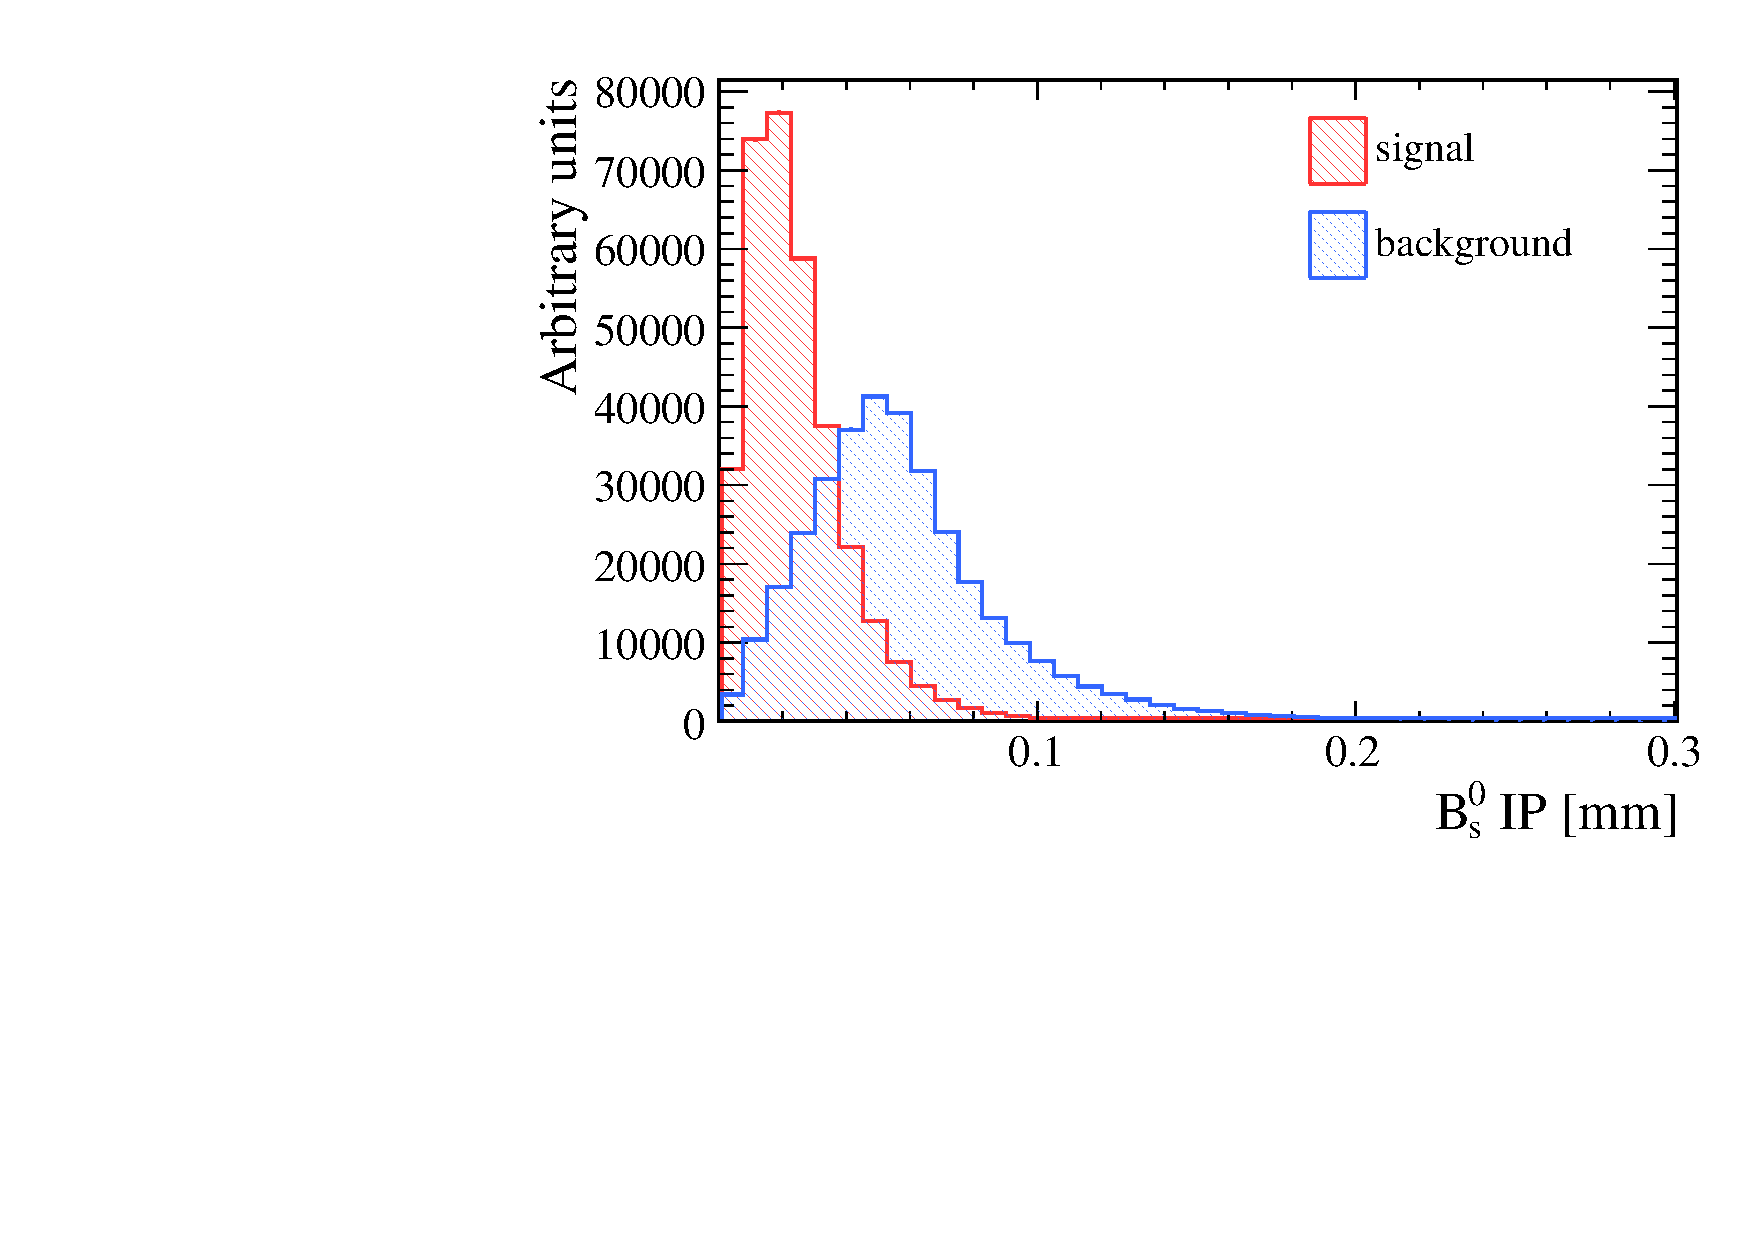
\includegraphics[width=0.49\textwidth]{./Figs/Appendix2/B_IP.pdf}
    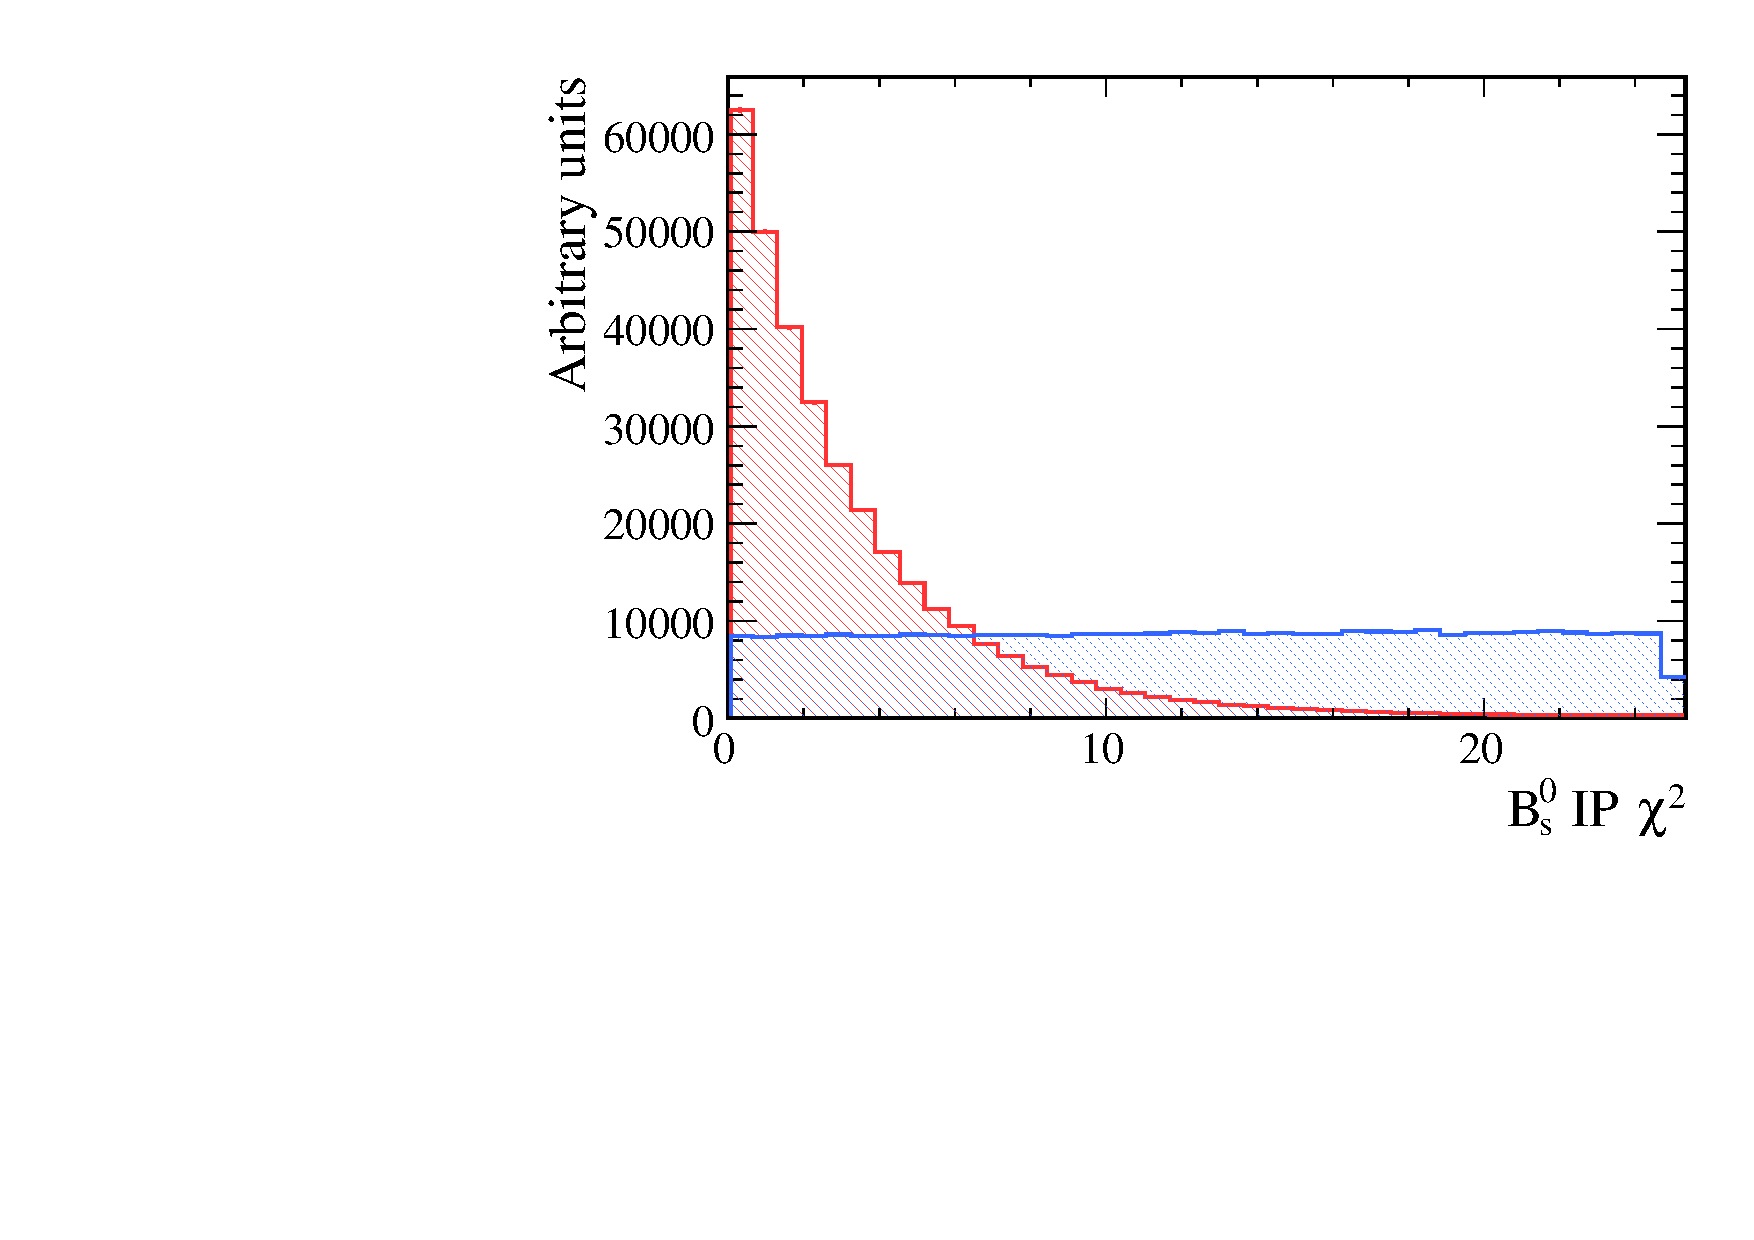
\includegraphics[width=0.49\textwidth]{./Figs/Appendix2/B_IPCHI2.pdf}
    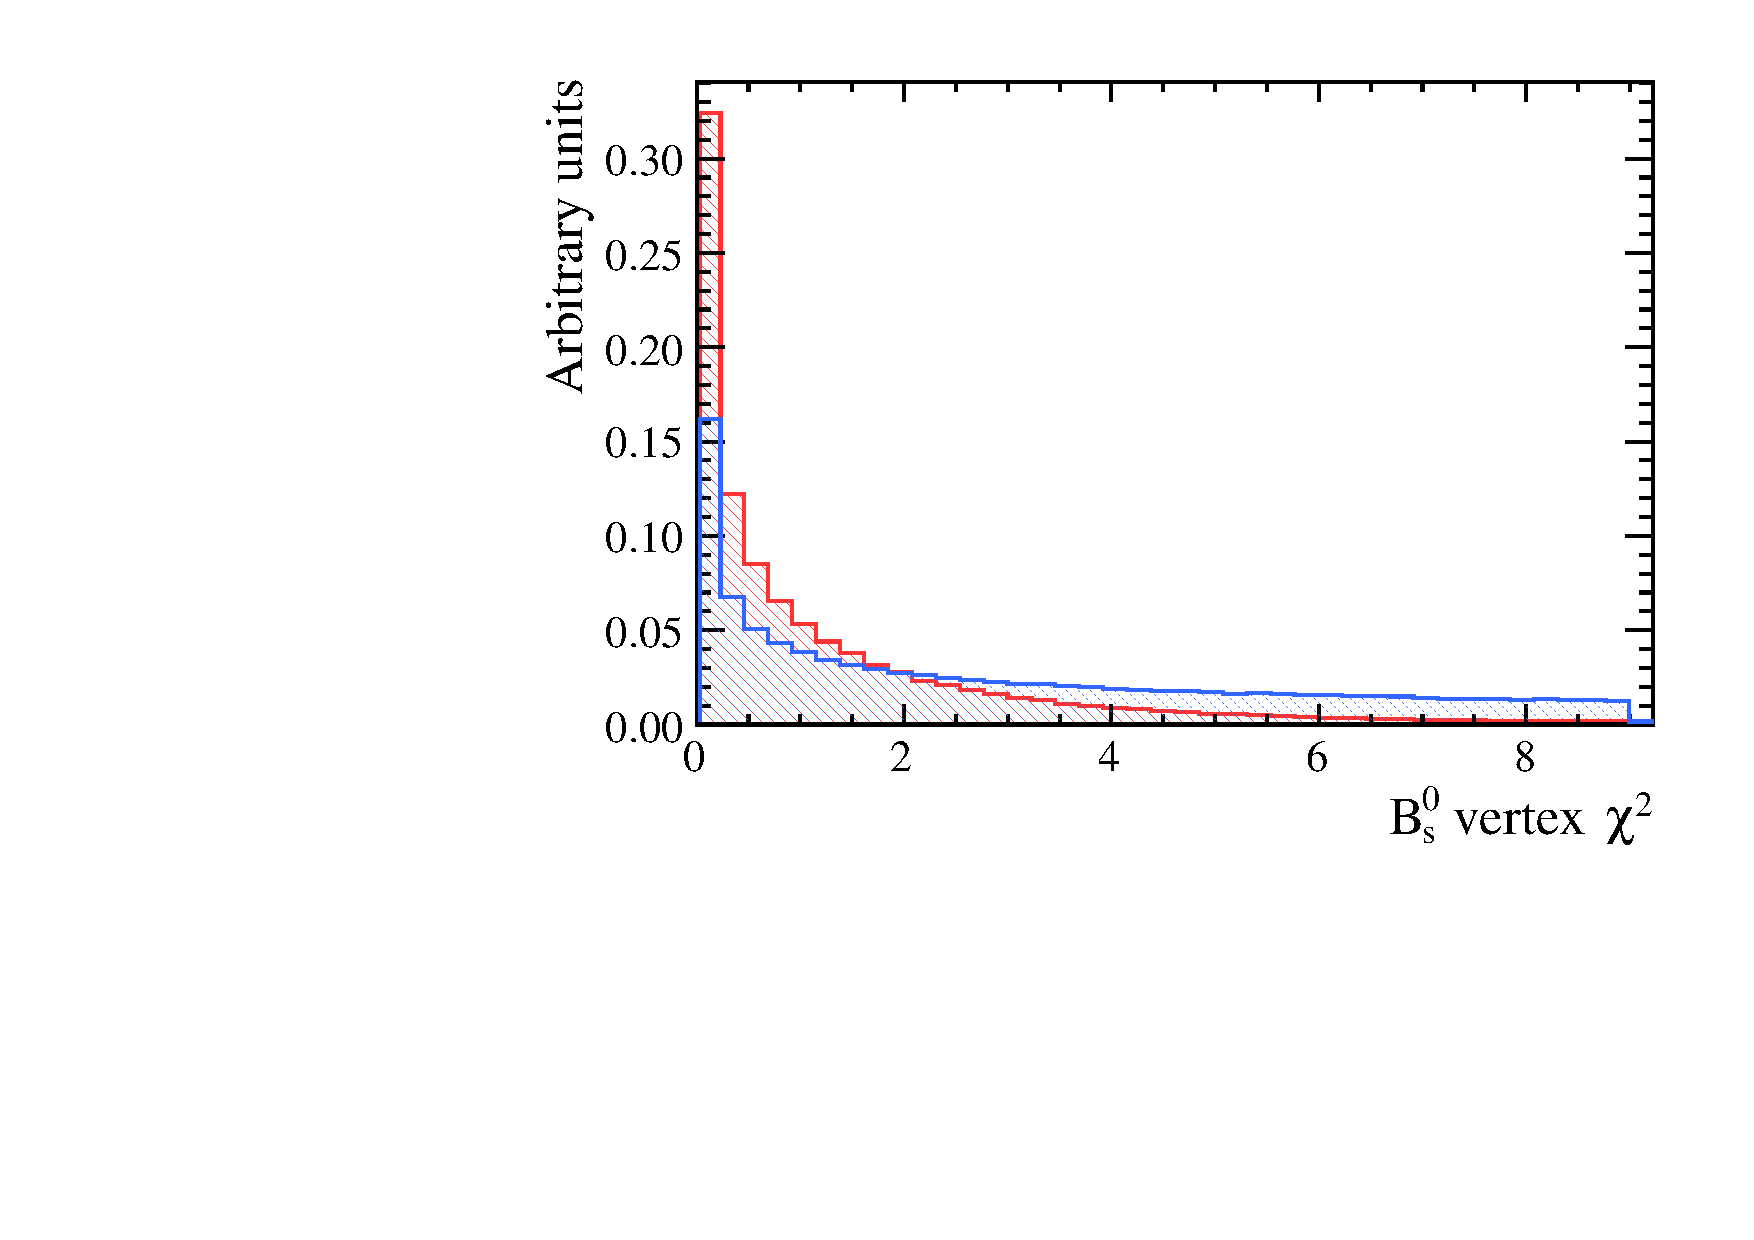
\includegraphics[width=0.49\textwidth]{./Figs/Appendix2/vertex.pdf}
    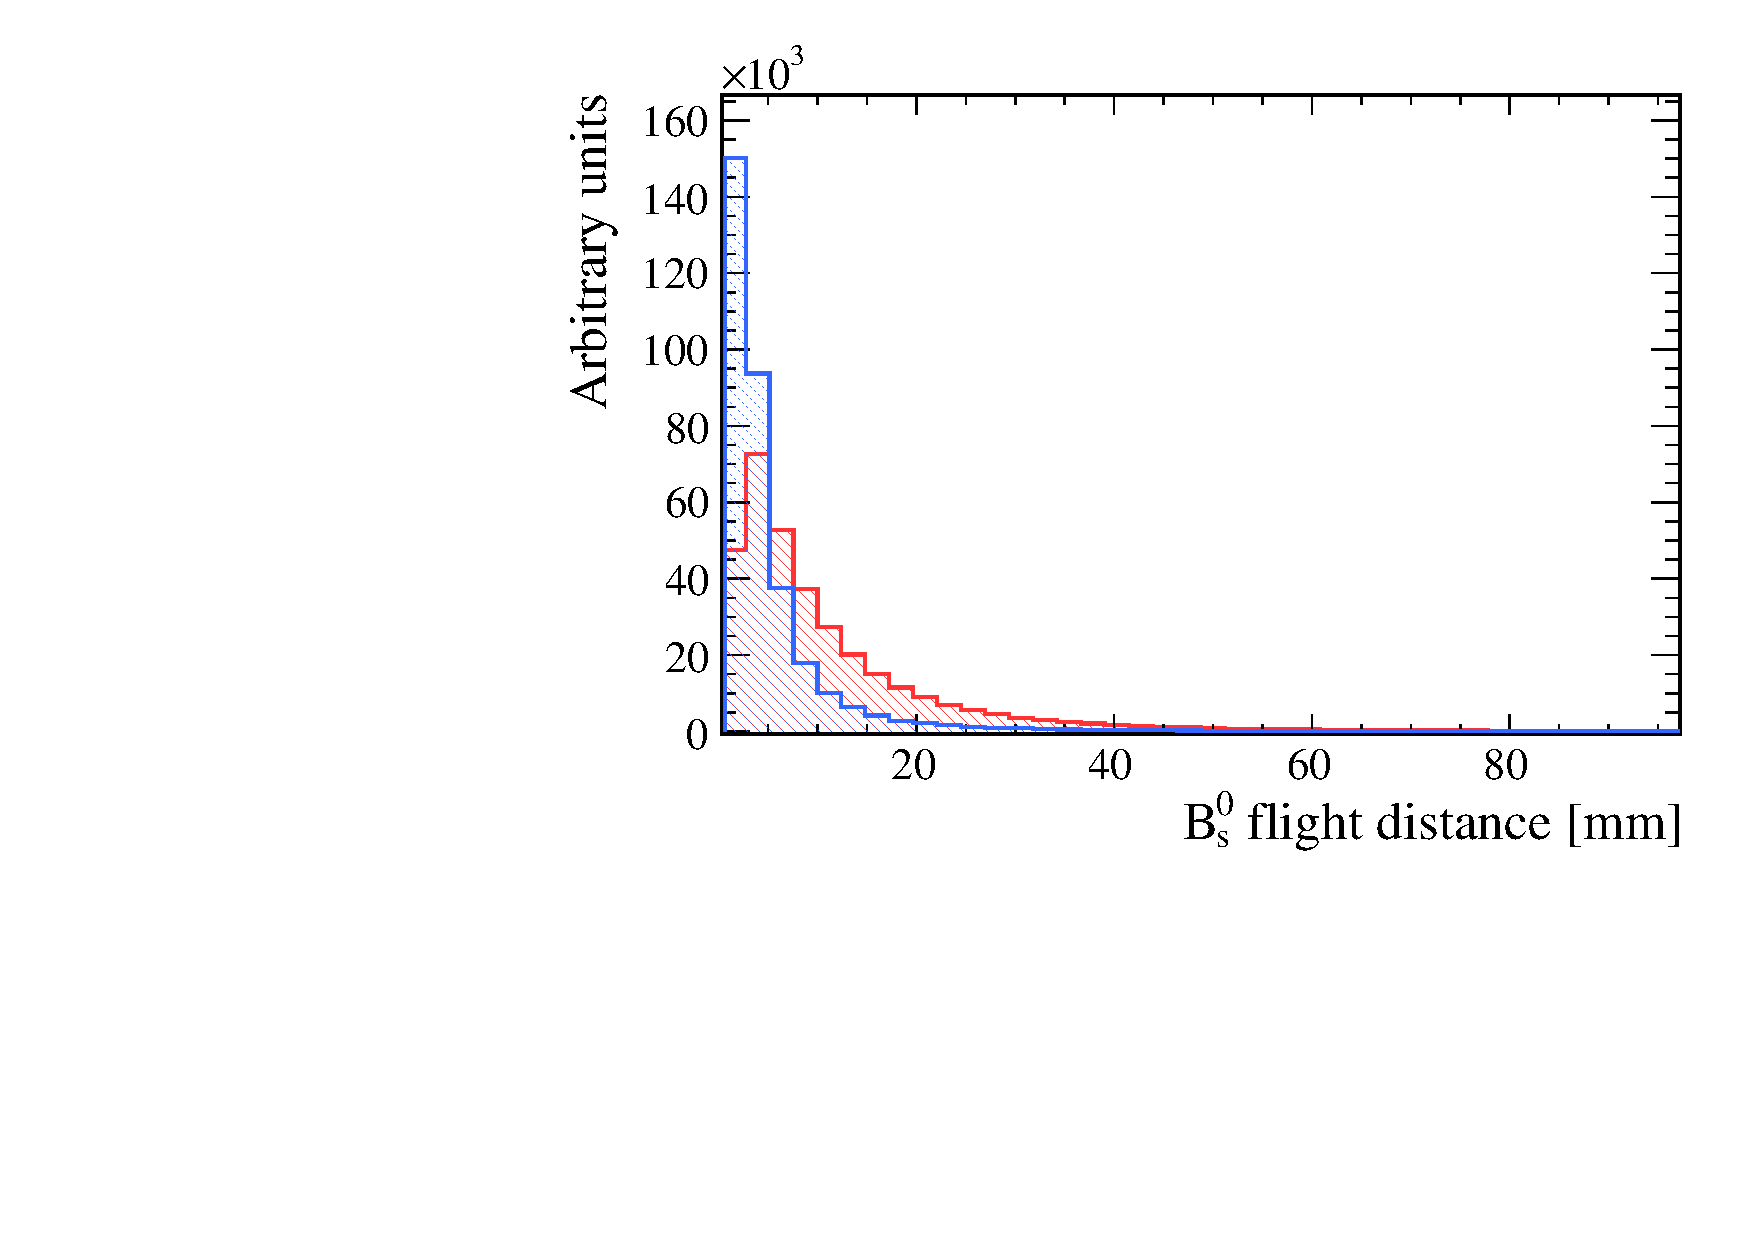
\includegraphics[width=0.49\textwidth]{./Figs/Appendix2/FD.pdf}
    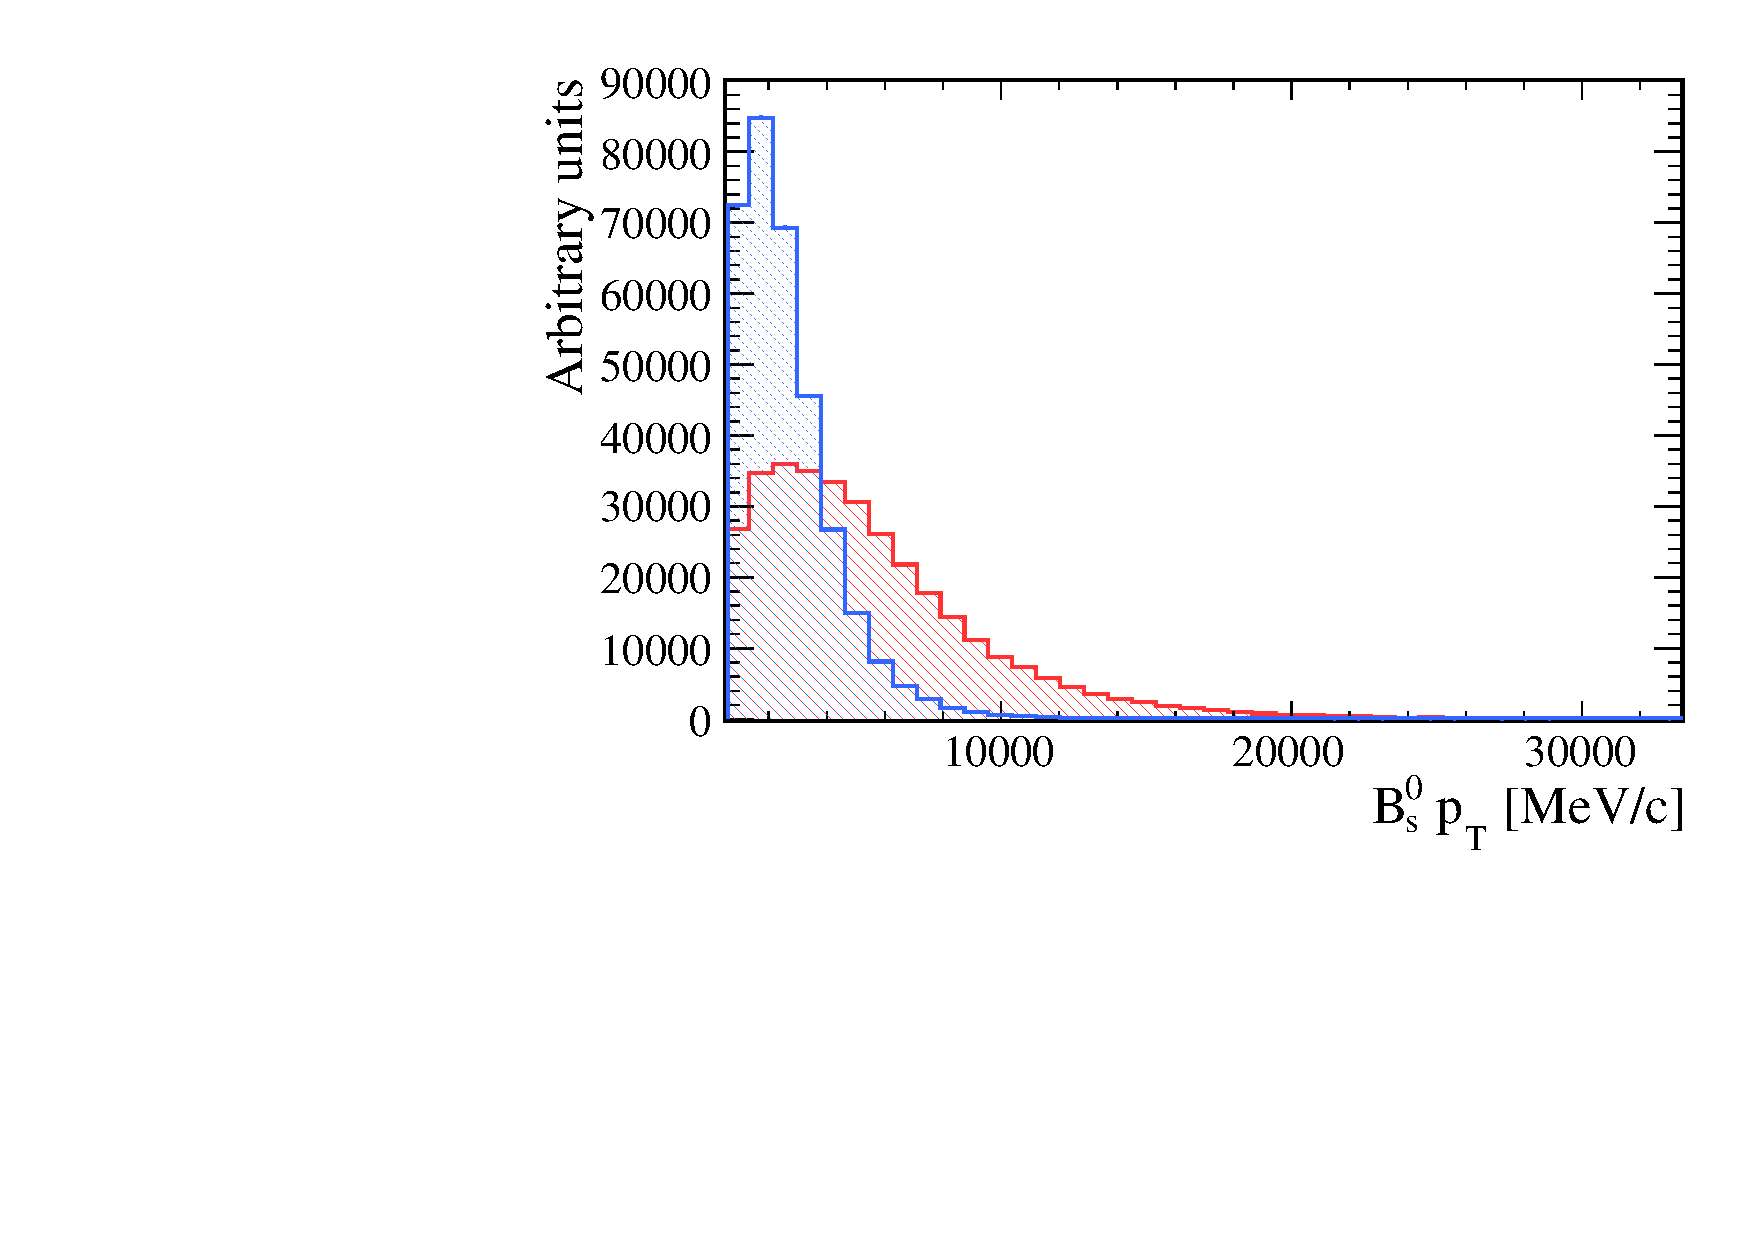
\includegraphics[width=0.49\textwidth]{./Figs/Appendix2/B_PT.pdf}
    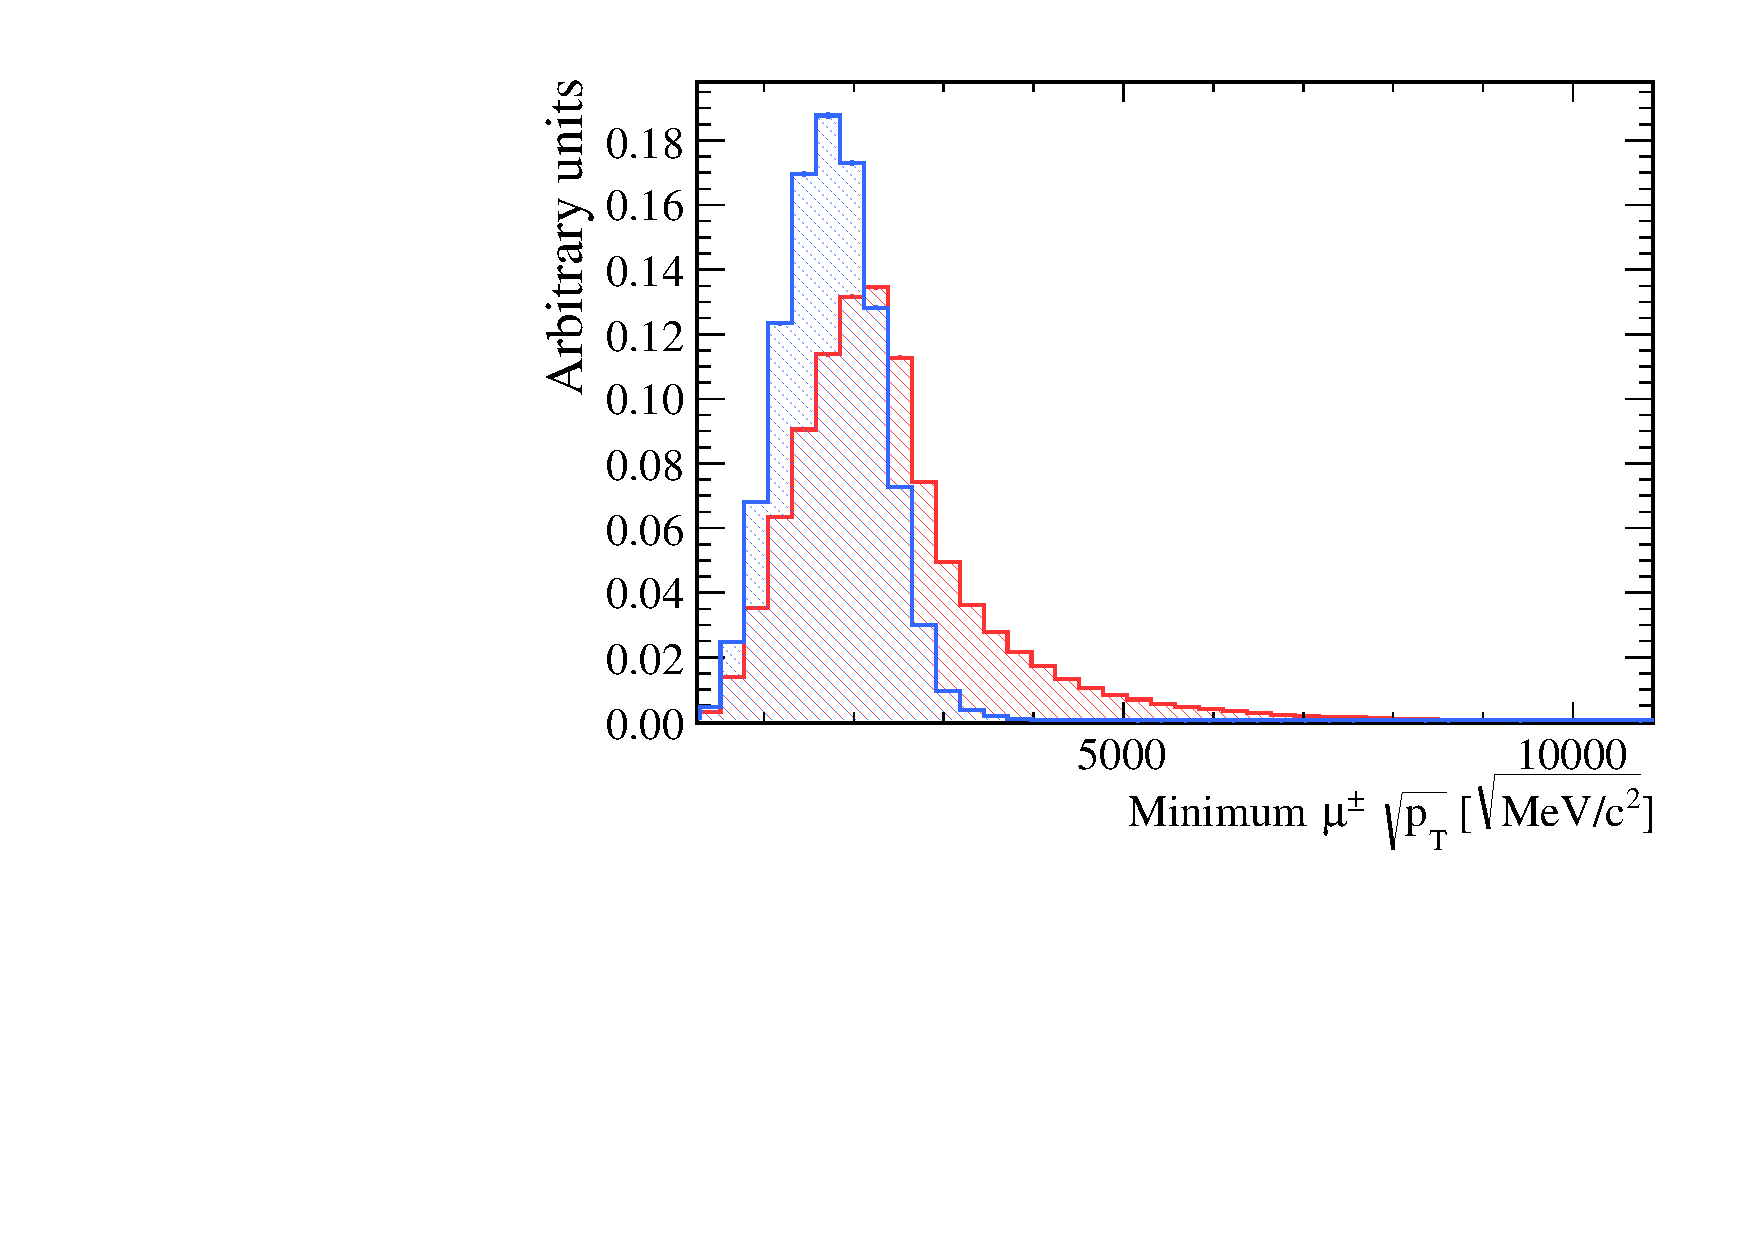
\includegraphics[width=0.49\textwidth]{./Figs/Appendix2/min_mu_PT.pdf}
    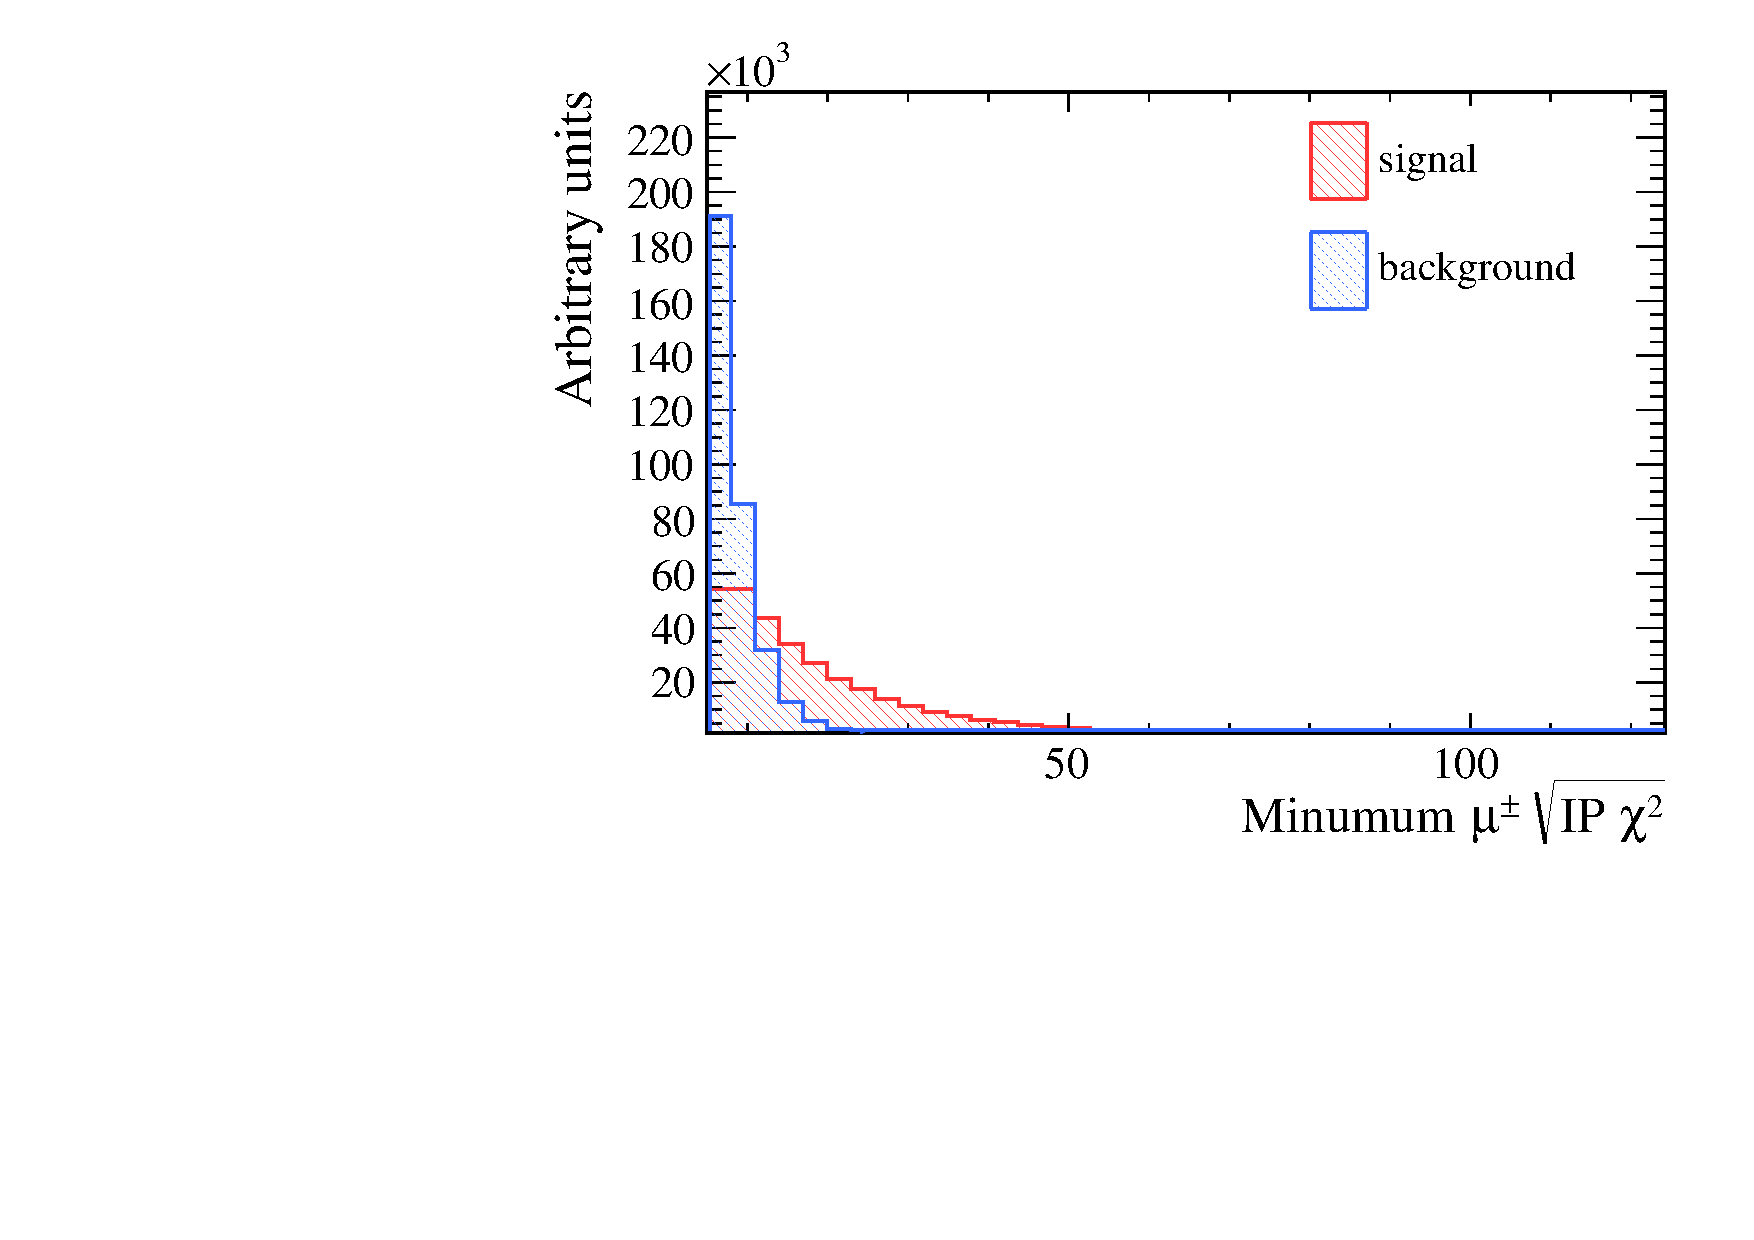
\includegraphics[width=0.49\textwidth]{./Figs/Appendix2/min_mu_IP.pdf}
    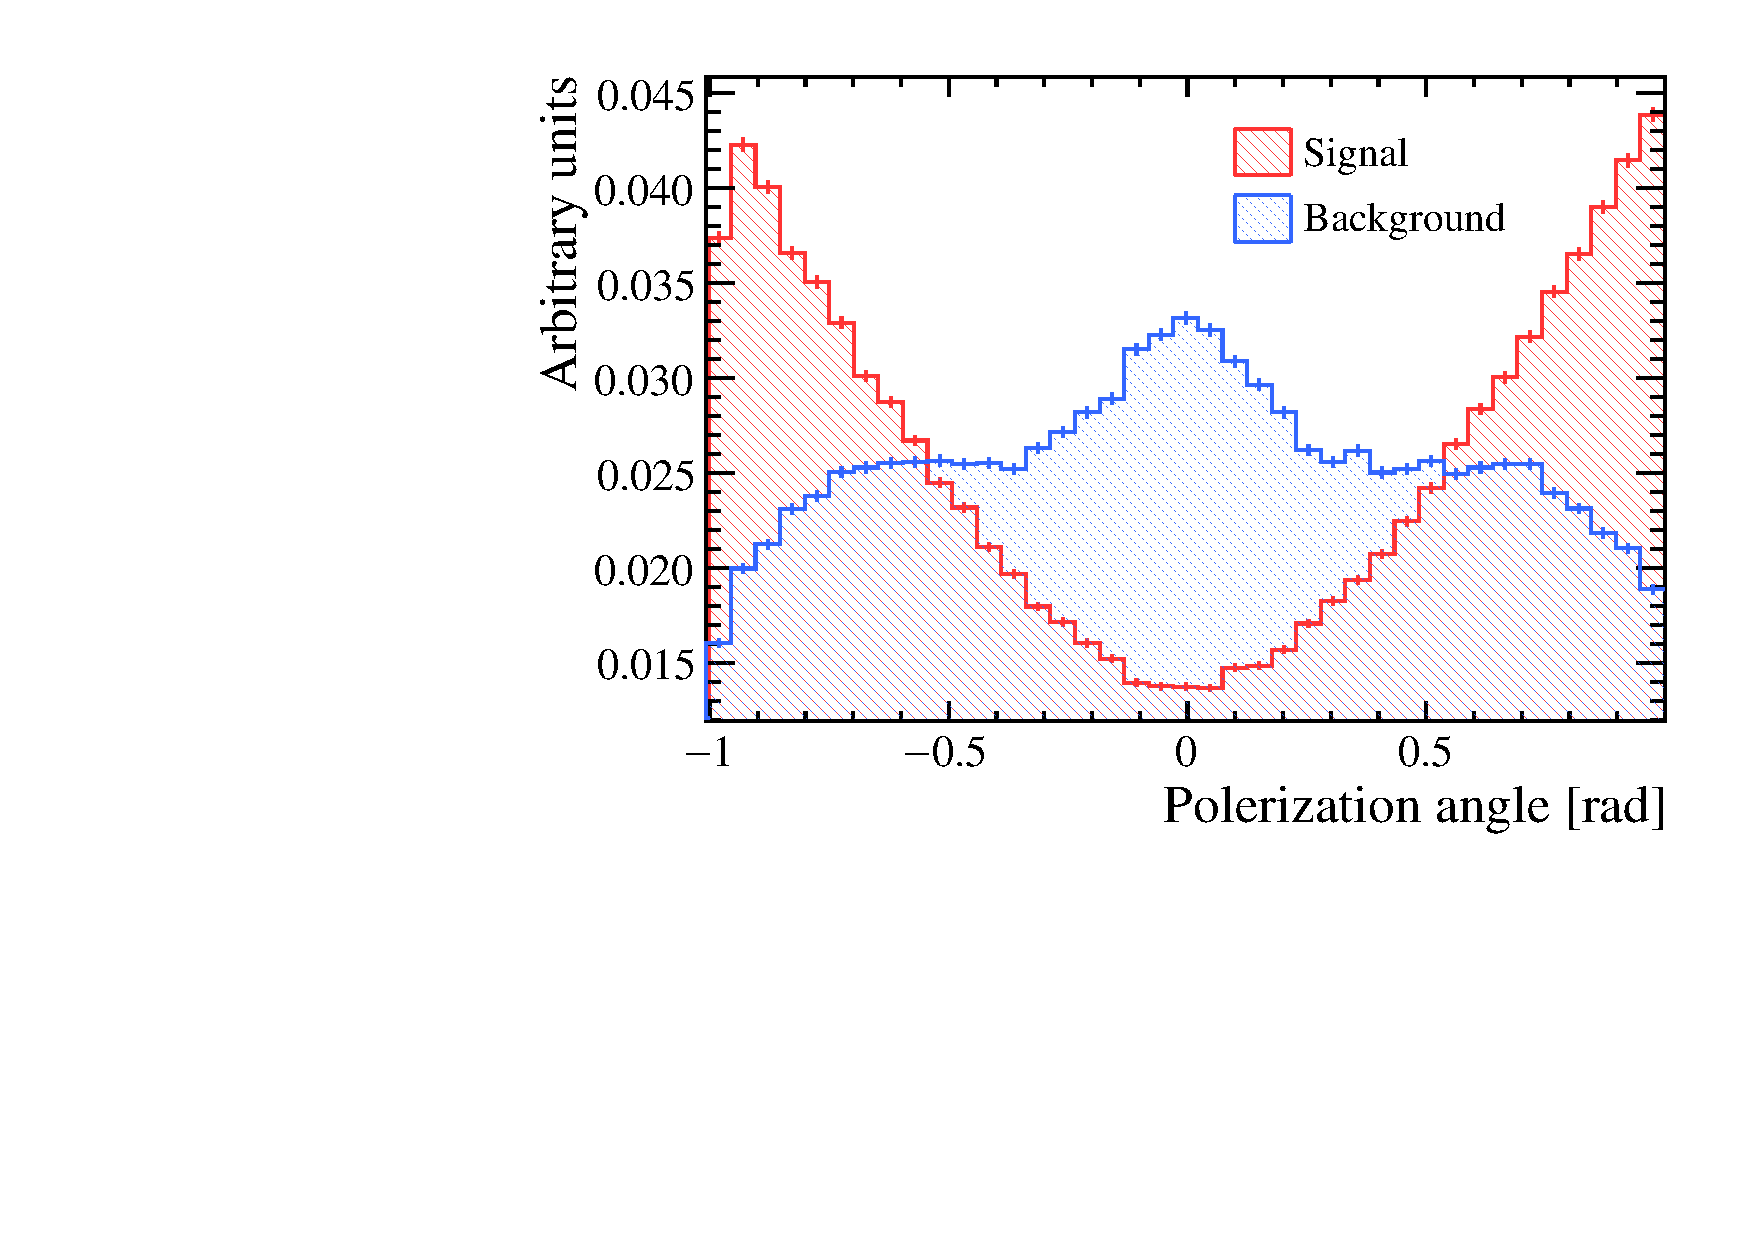
\includegraphics[width=0.49\textwidth]{./Figs/Appendix2/polerization.pdf}
  \caption{The distributions of the input variables used in the adaptive boost and uBoost BDTs for \bsmumu and \bbbarmumux 2012 simulated decays.}
  \label{fig:myBDTvars}
\end{figure}


\begin{figure}[htbp]
  \centering
    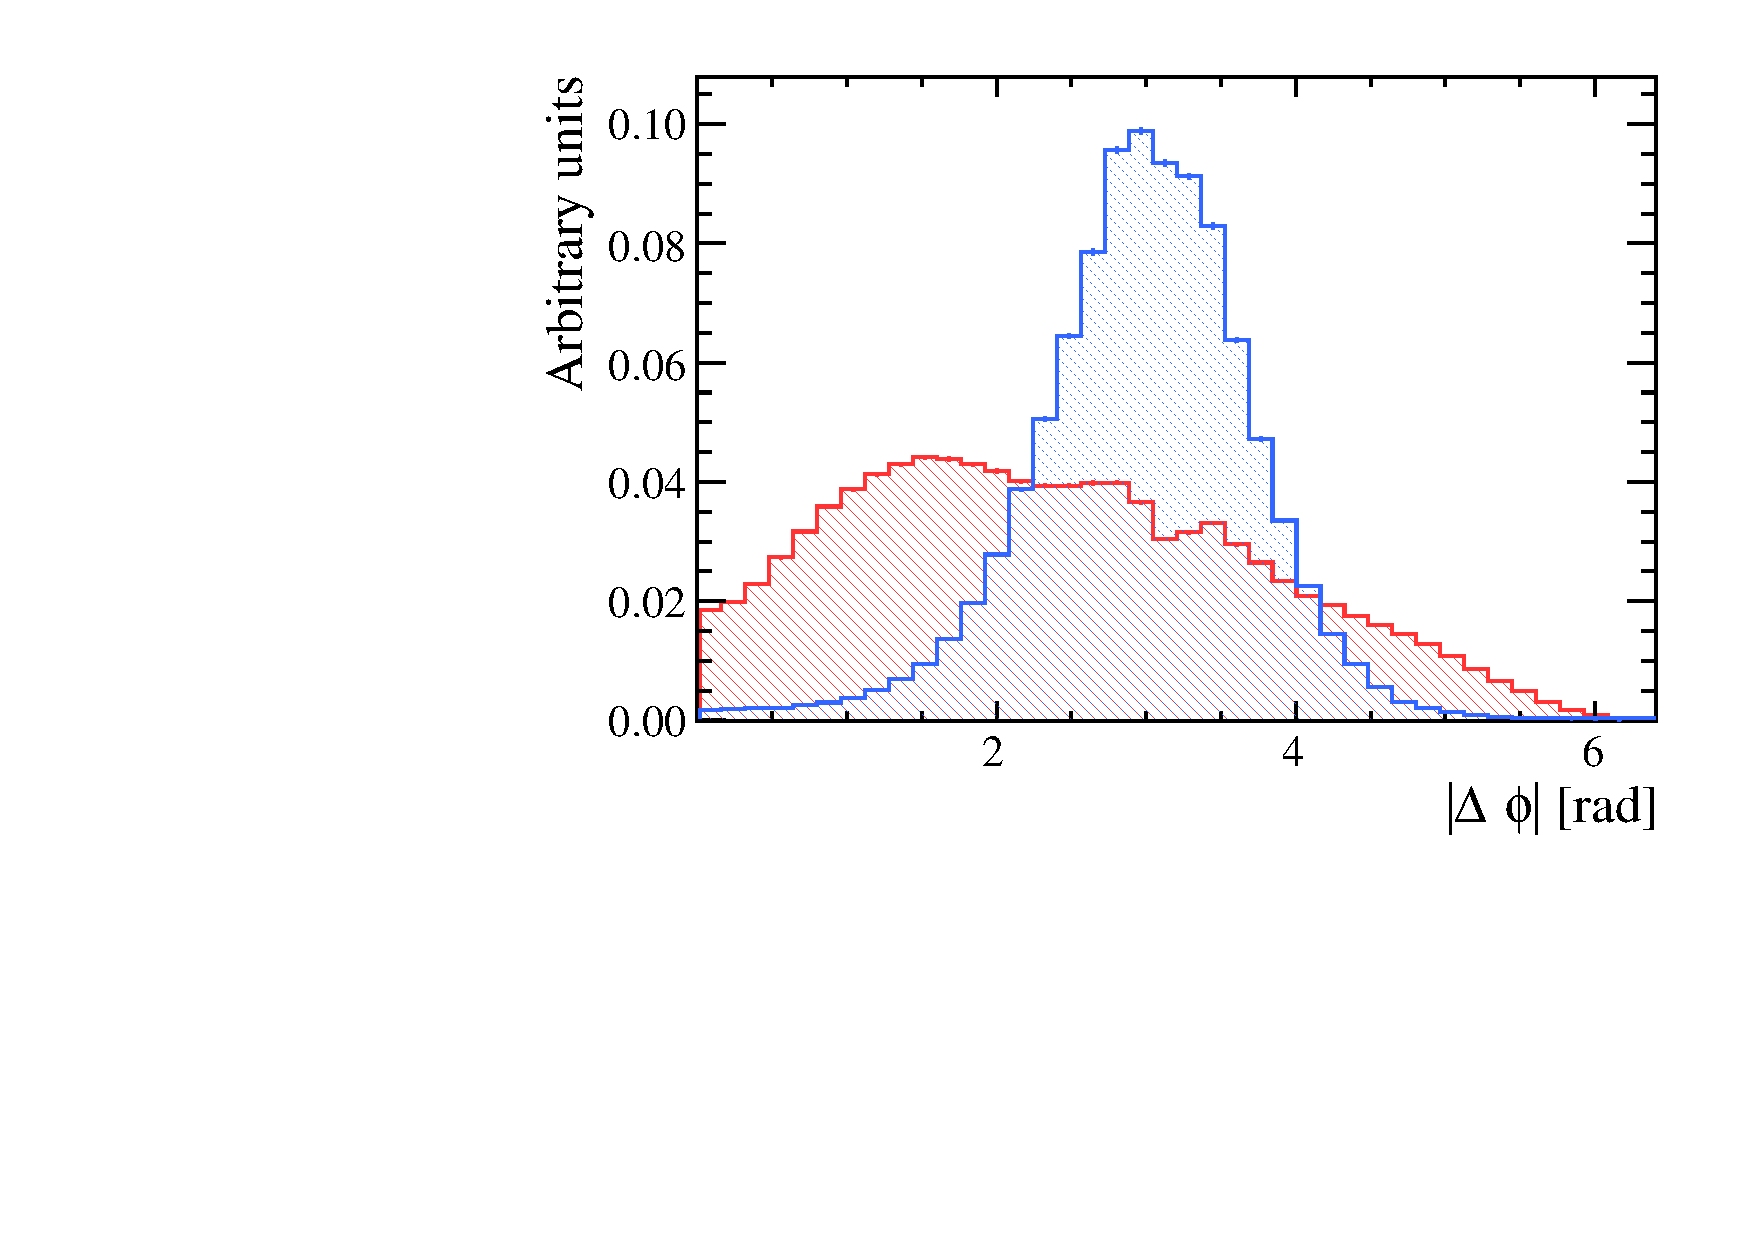
\includegraphics[width=0.49\textwidth]{./Figs/Appendix2/phi.pdf}
    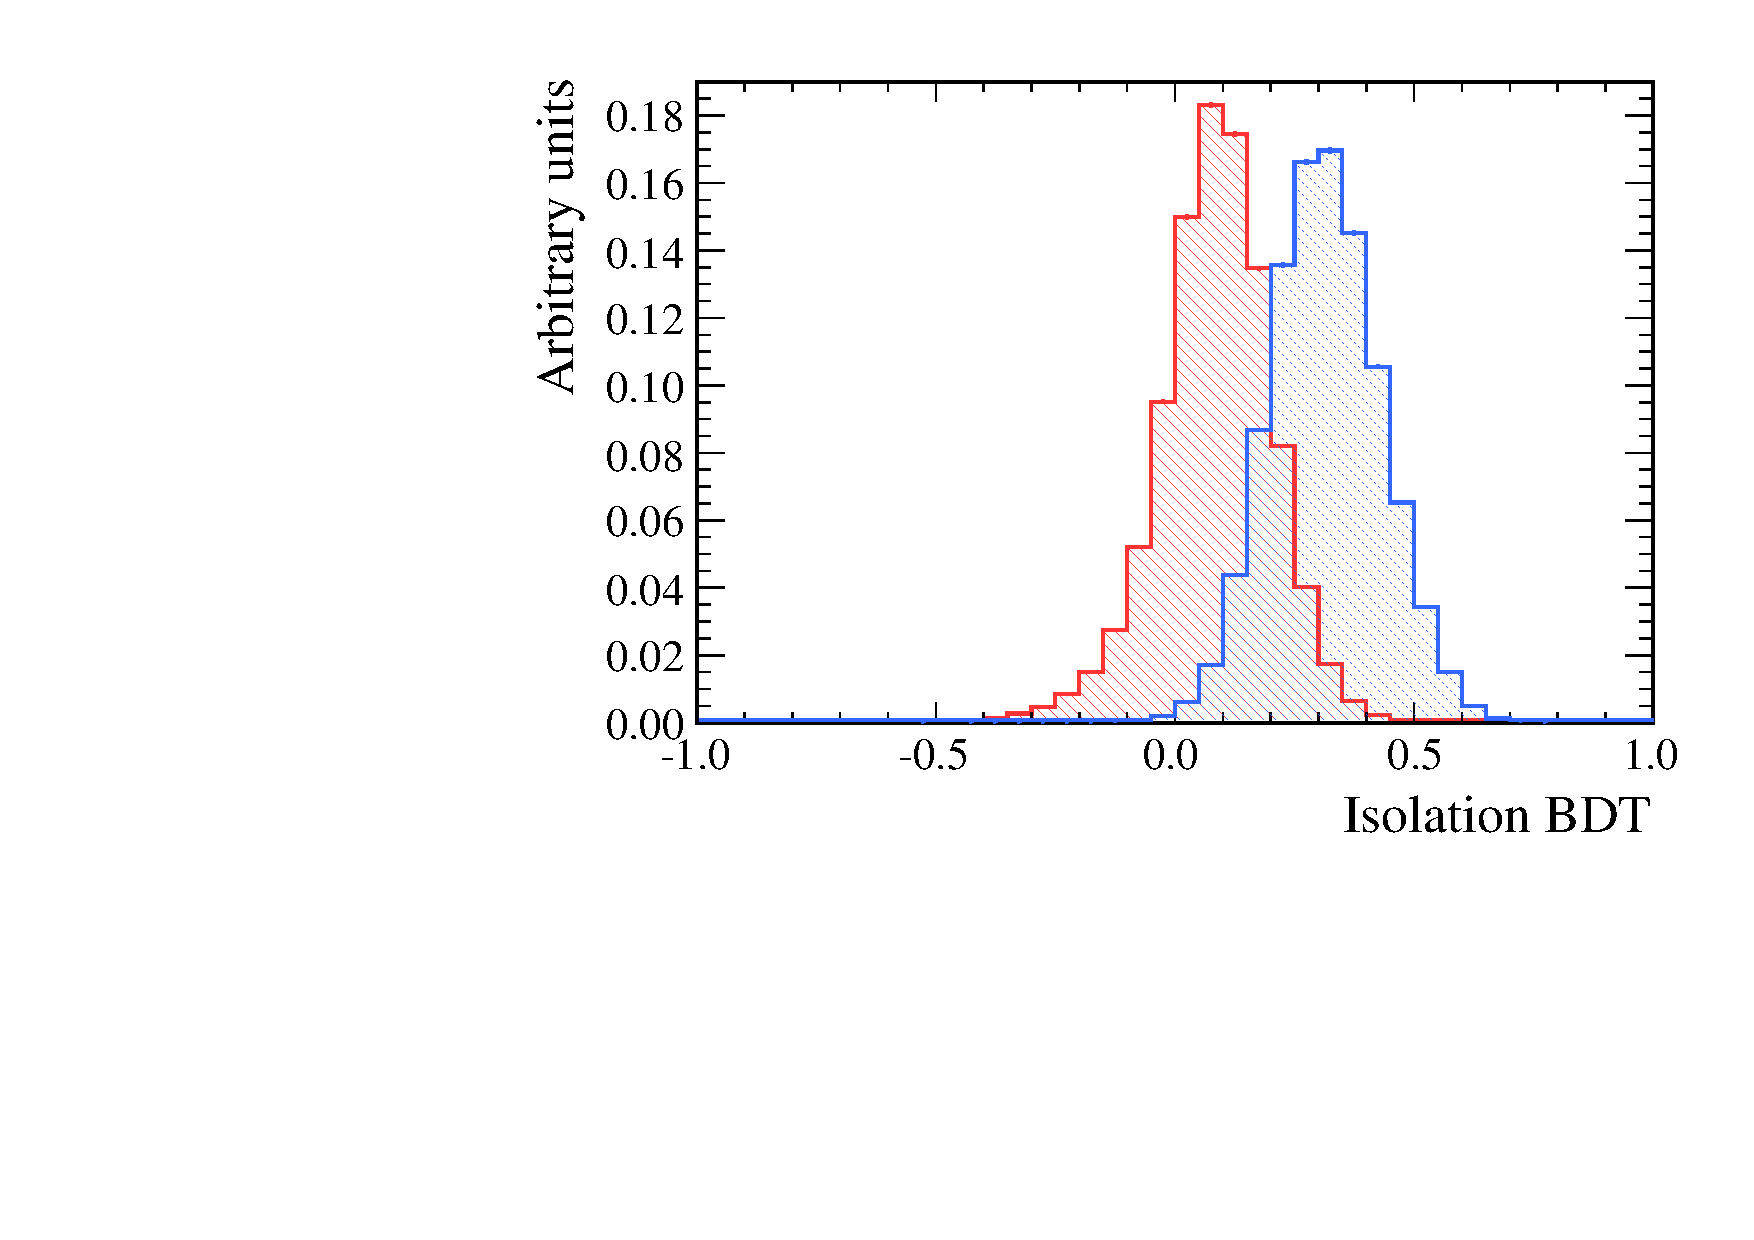
\includegraphics[width=0.49\textwidth]{./Figs/Appendix2/isoBDT.pdf}
    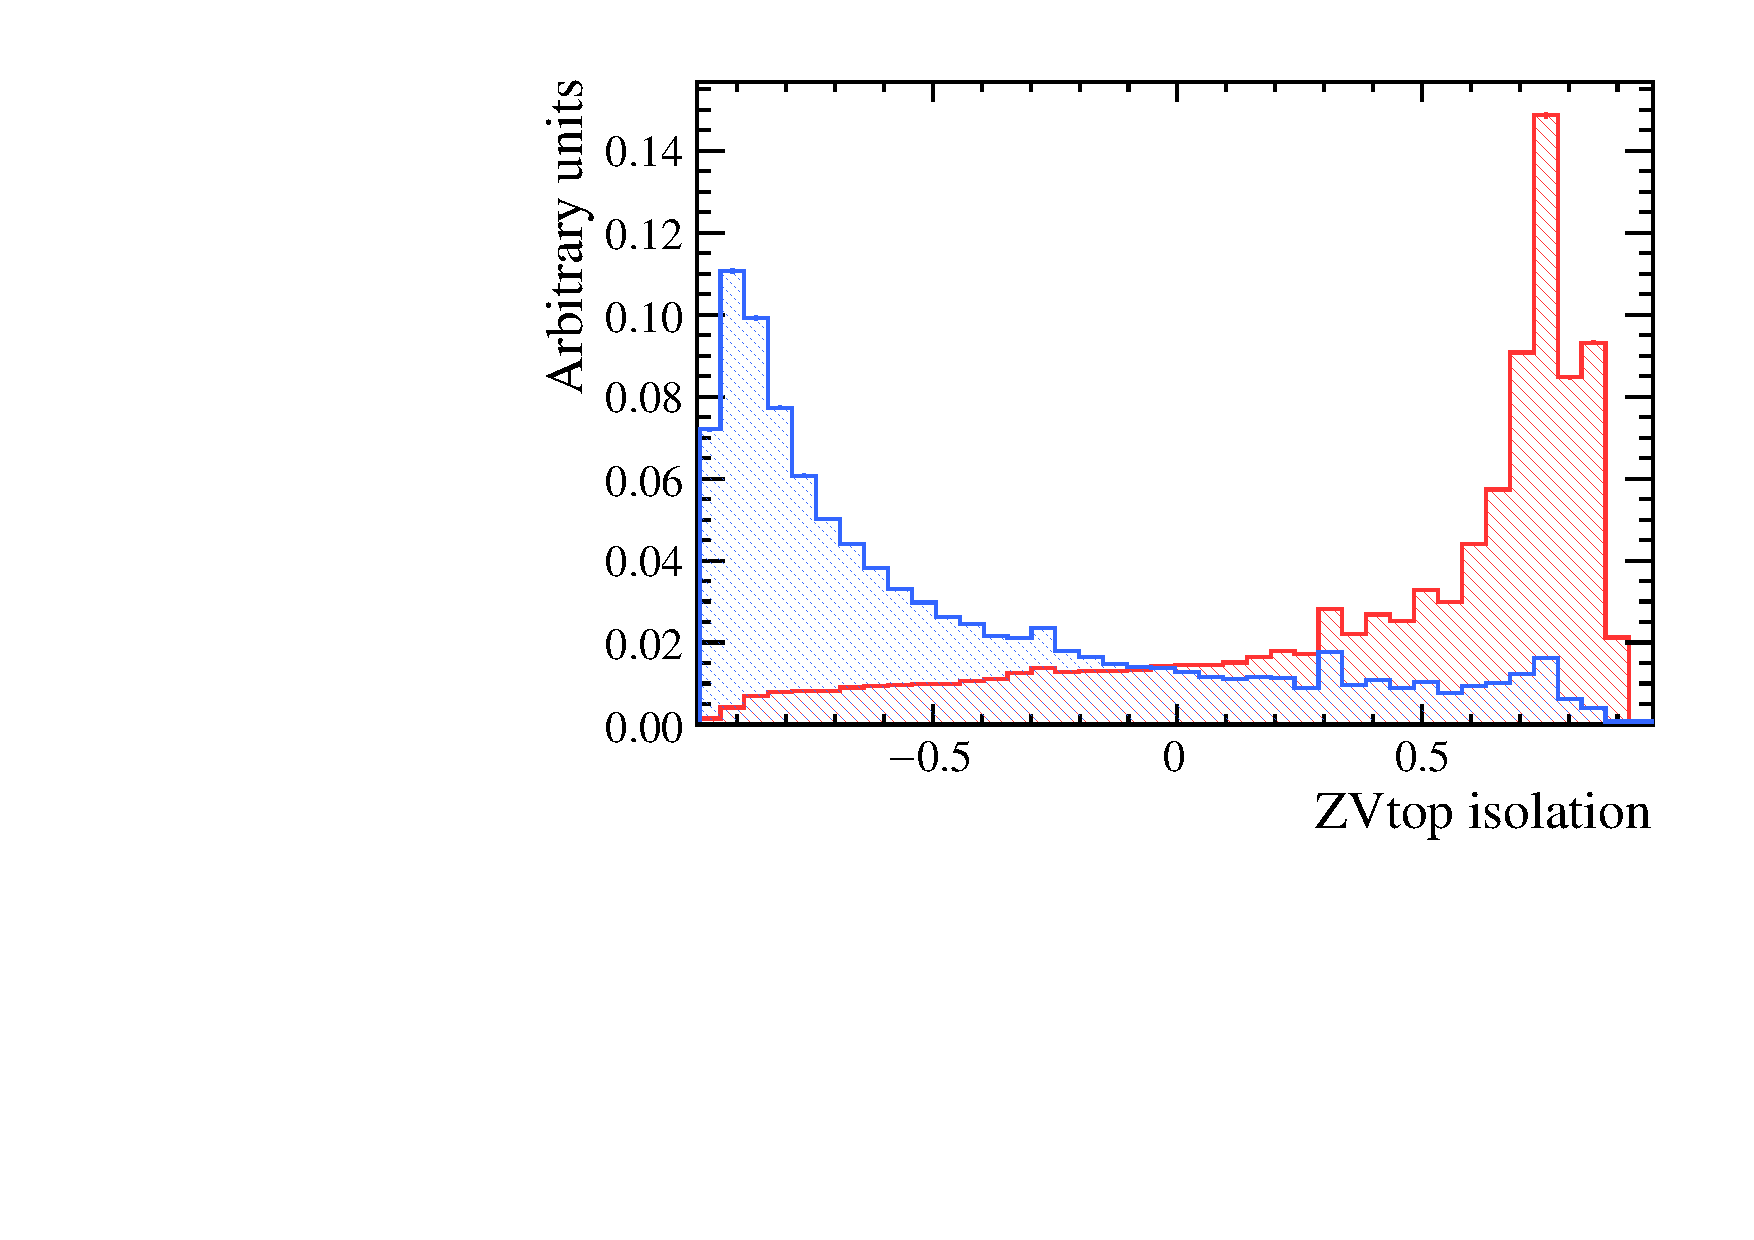
\includegraphics[width=0.49\textwidth]{./Figs/Appendix2/ZViso.pdf}
    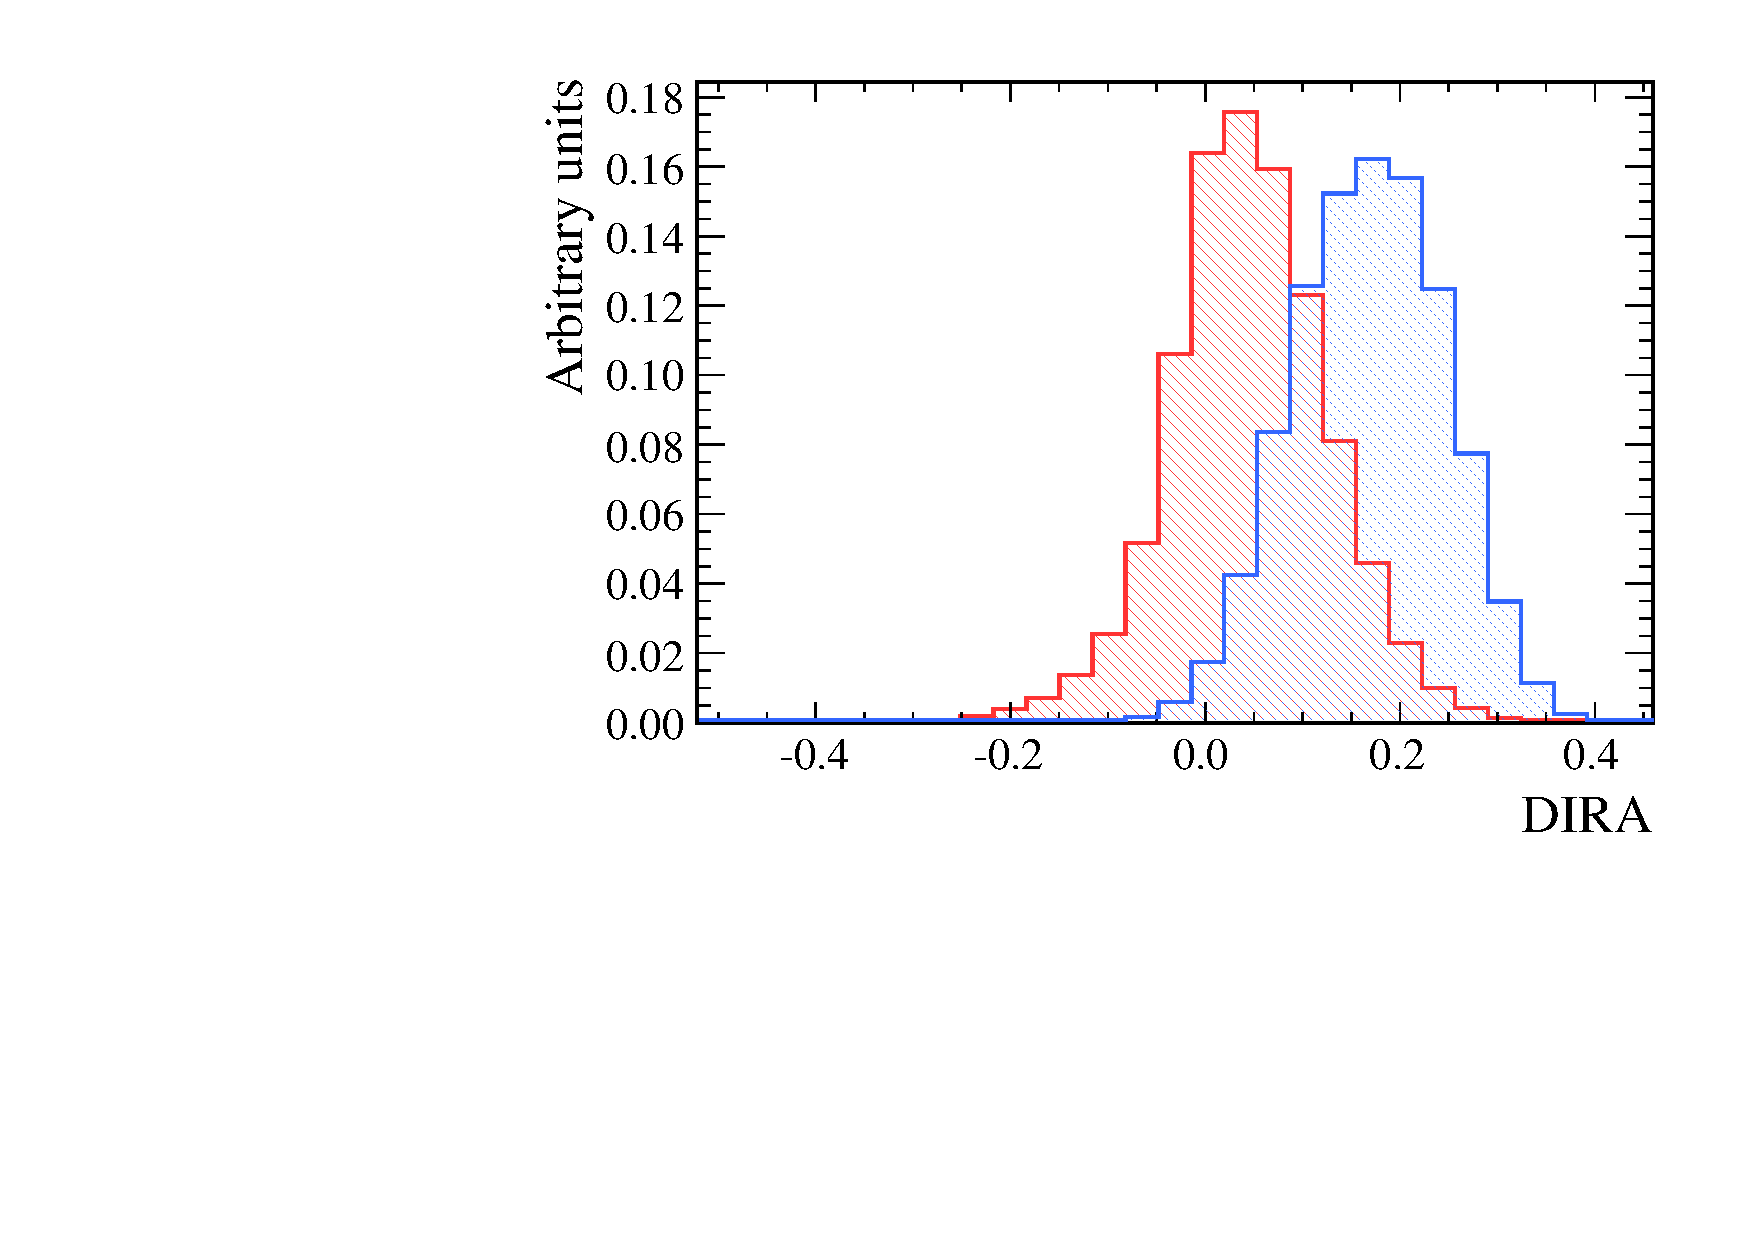
\includegraphics[width=0.49\textwidth]{./Figs/Appendix2/DIRA.pdf}
    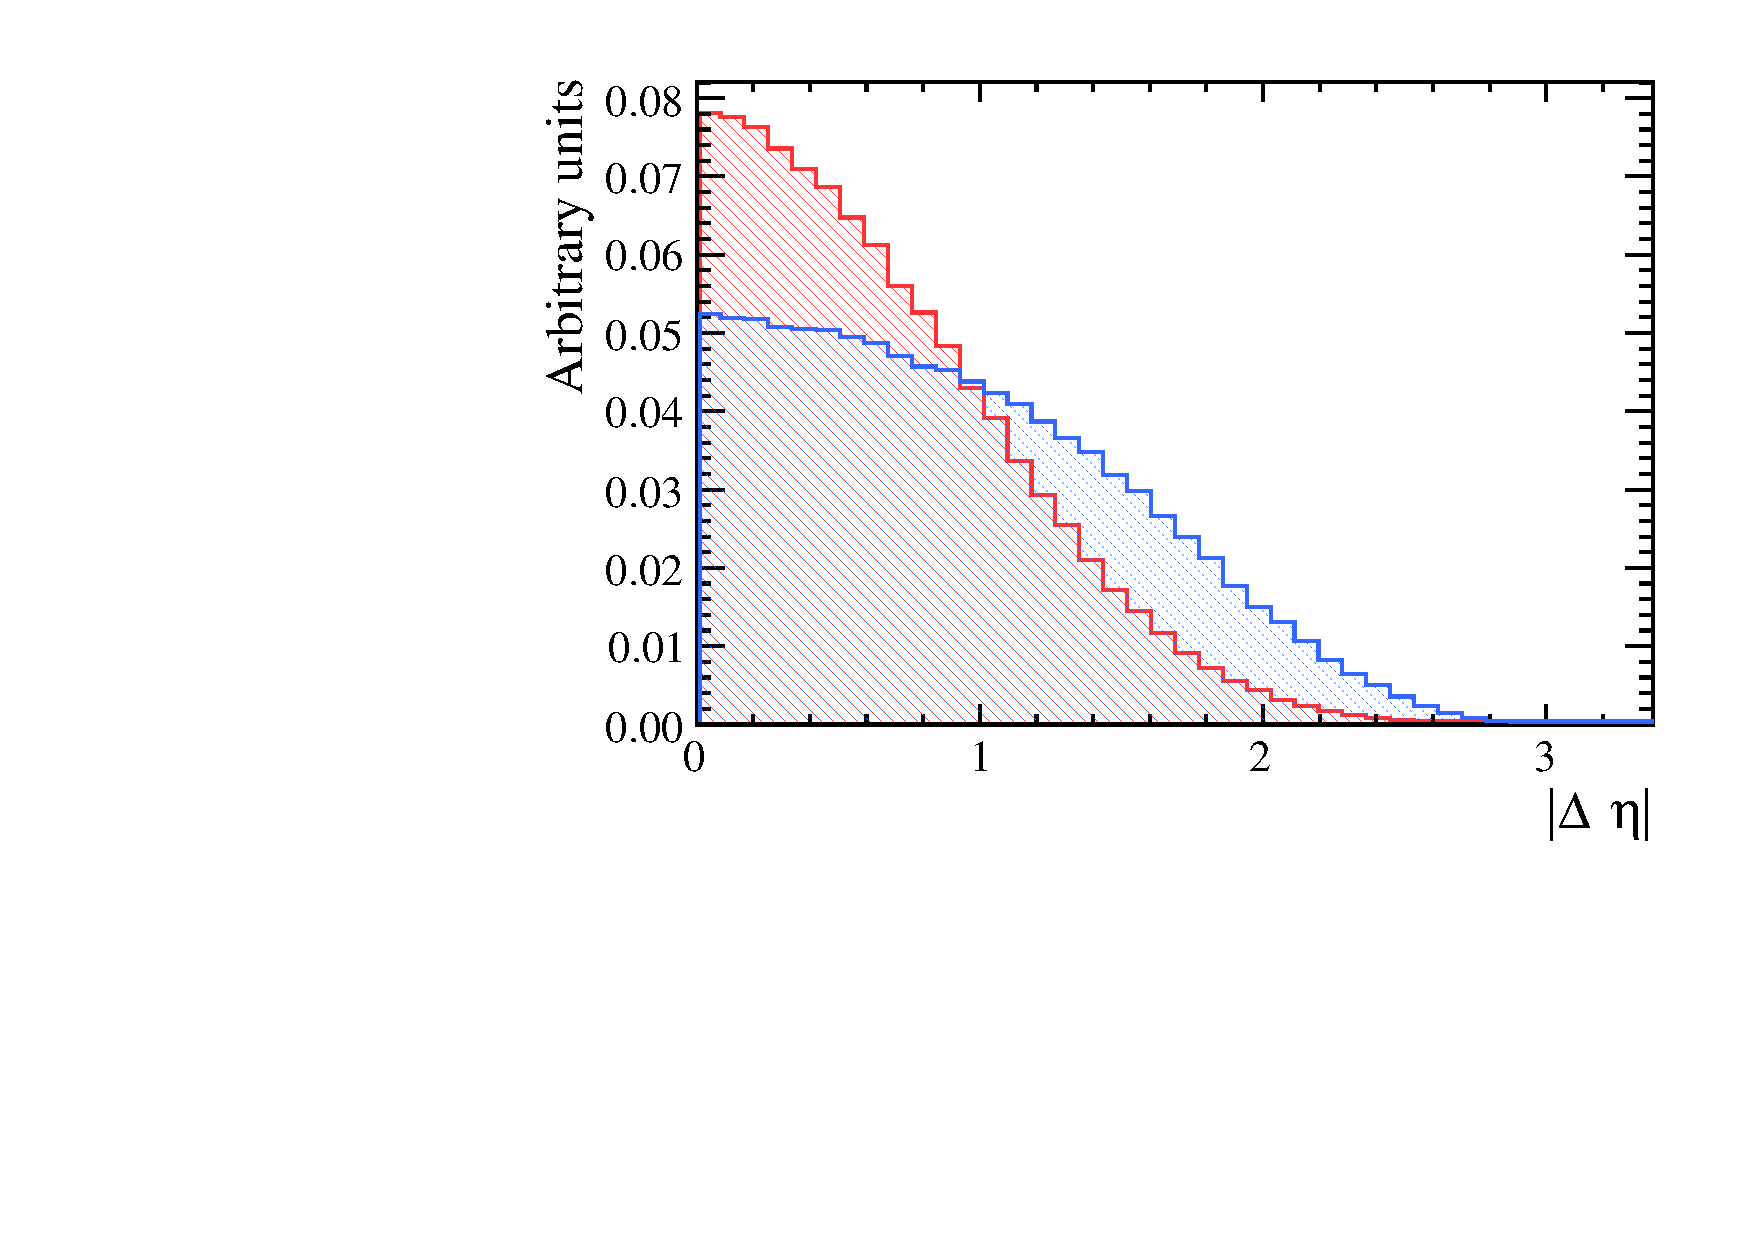
\includegraphics[width=0.49\textwidth]{./Figs/Appendix2/eta.pdf}
    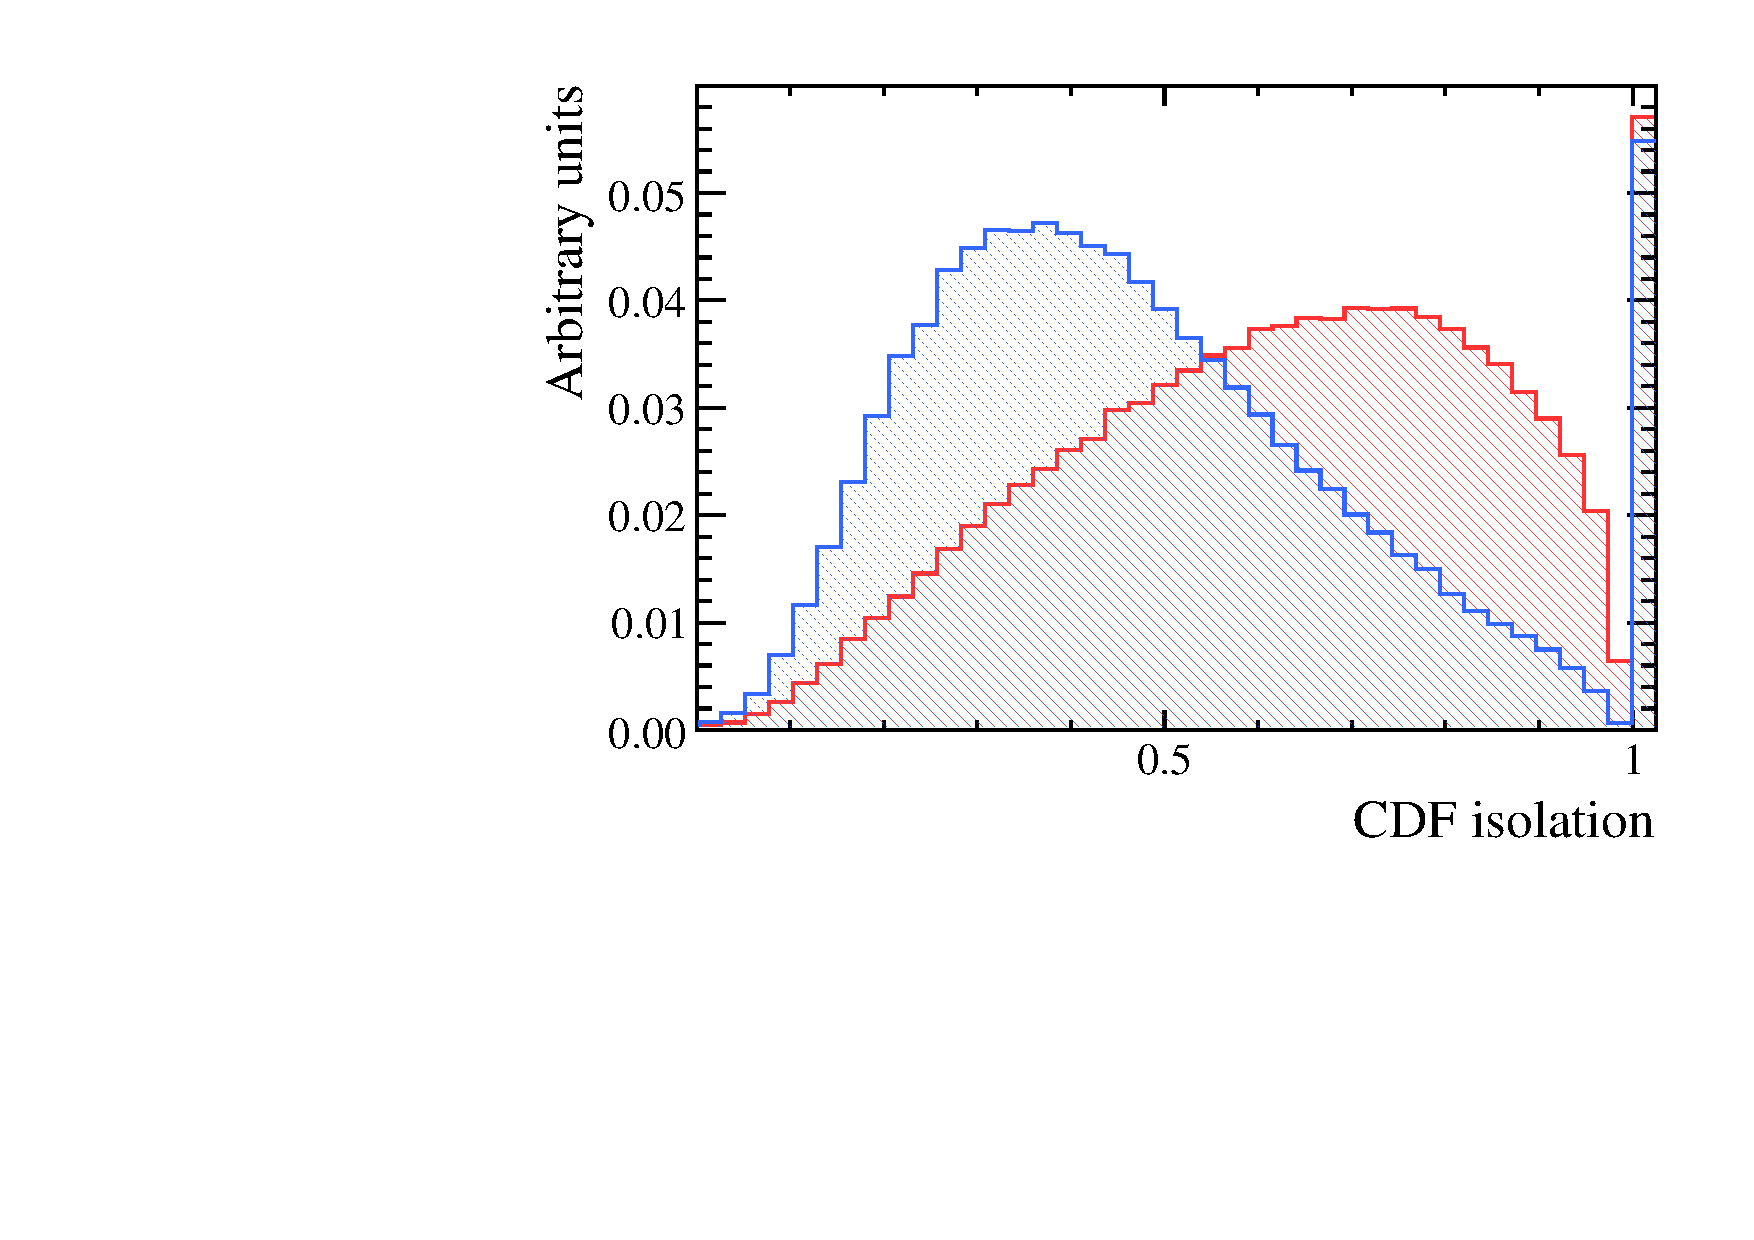
\includegraphics[width=0.49\textwidth]{./Figs/Appendix2/CDF.pdf}
    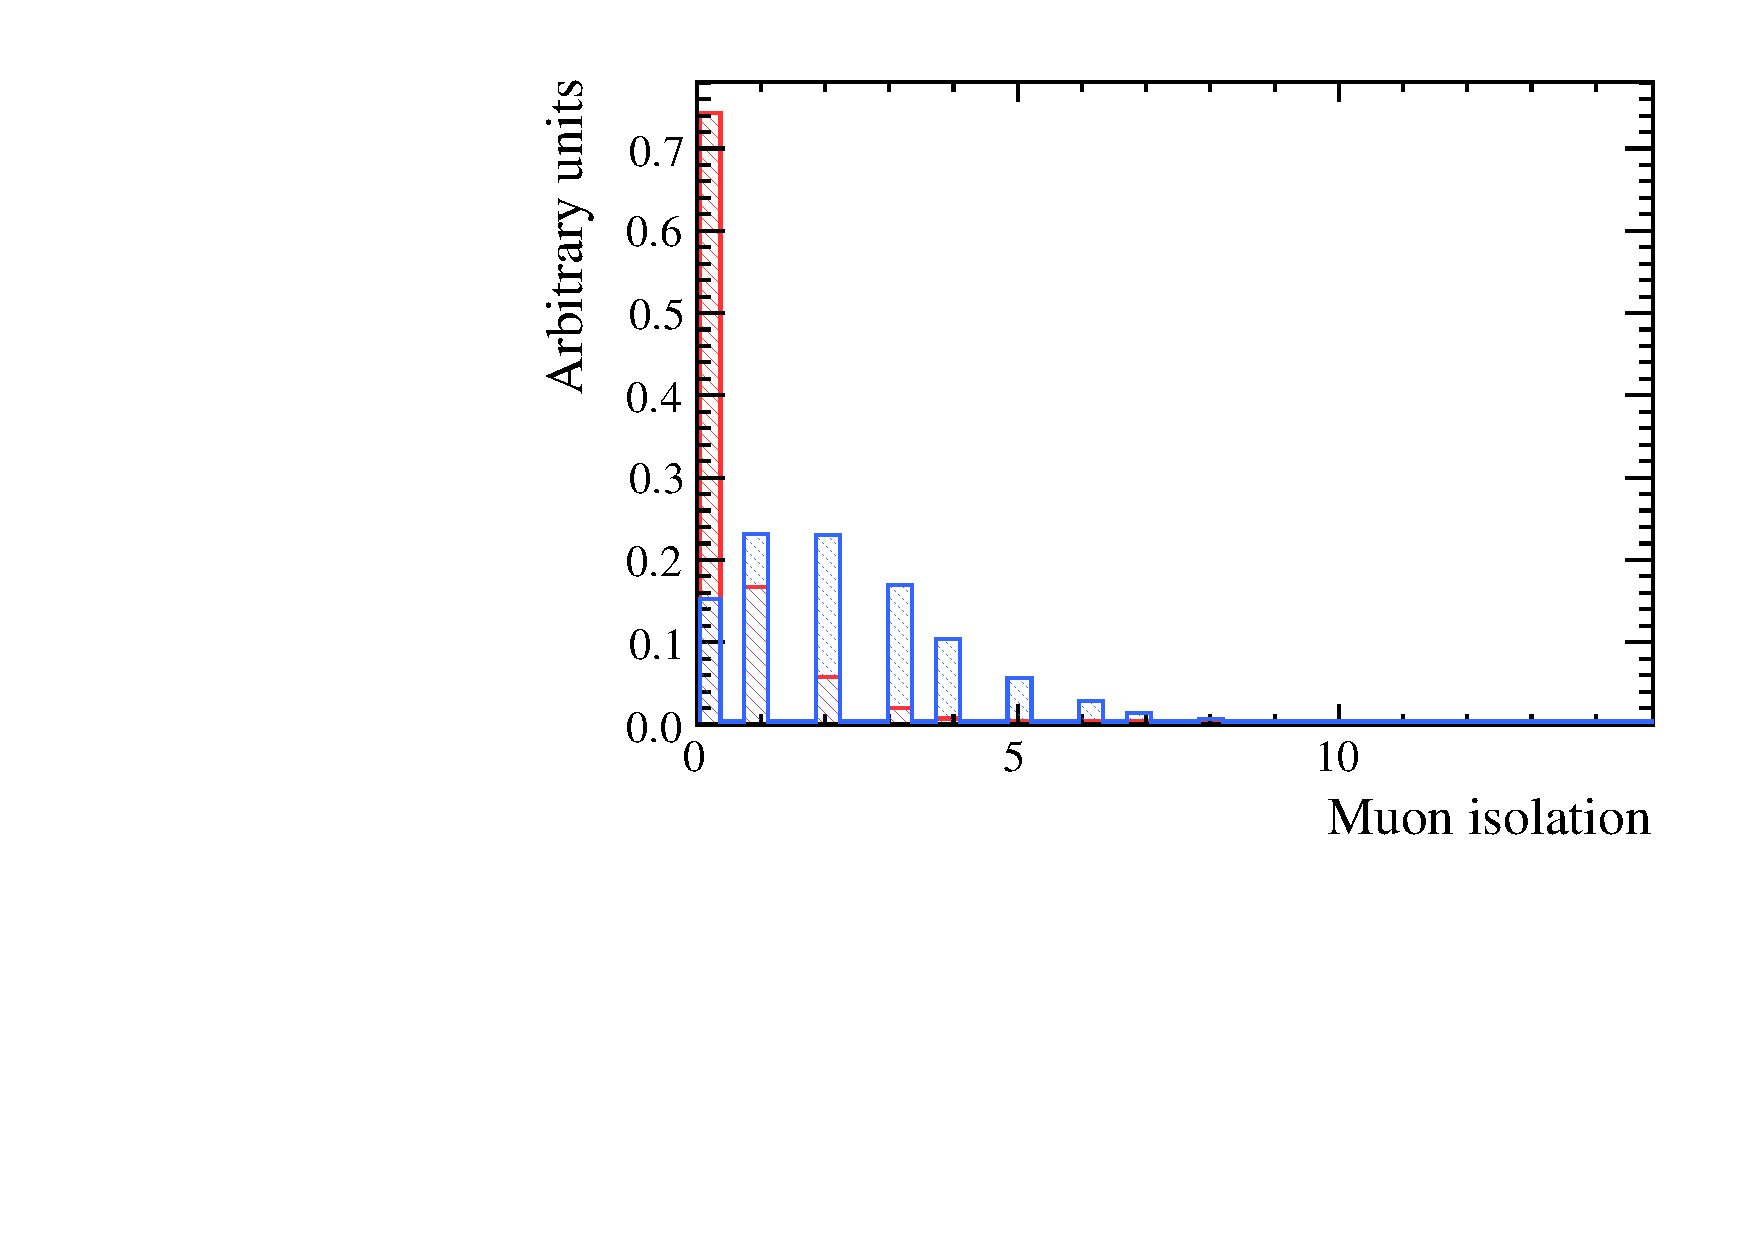
\includegraphics[width=0.49\textwidth]{./Figs/Appendix2/muon_iso.pdf}
    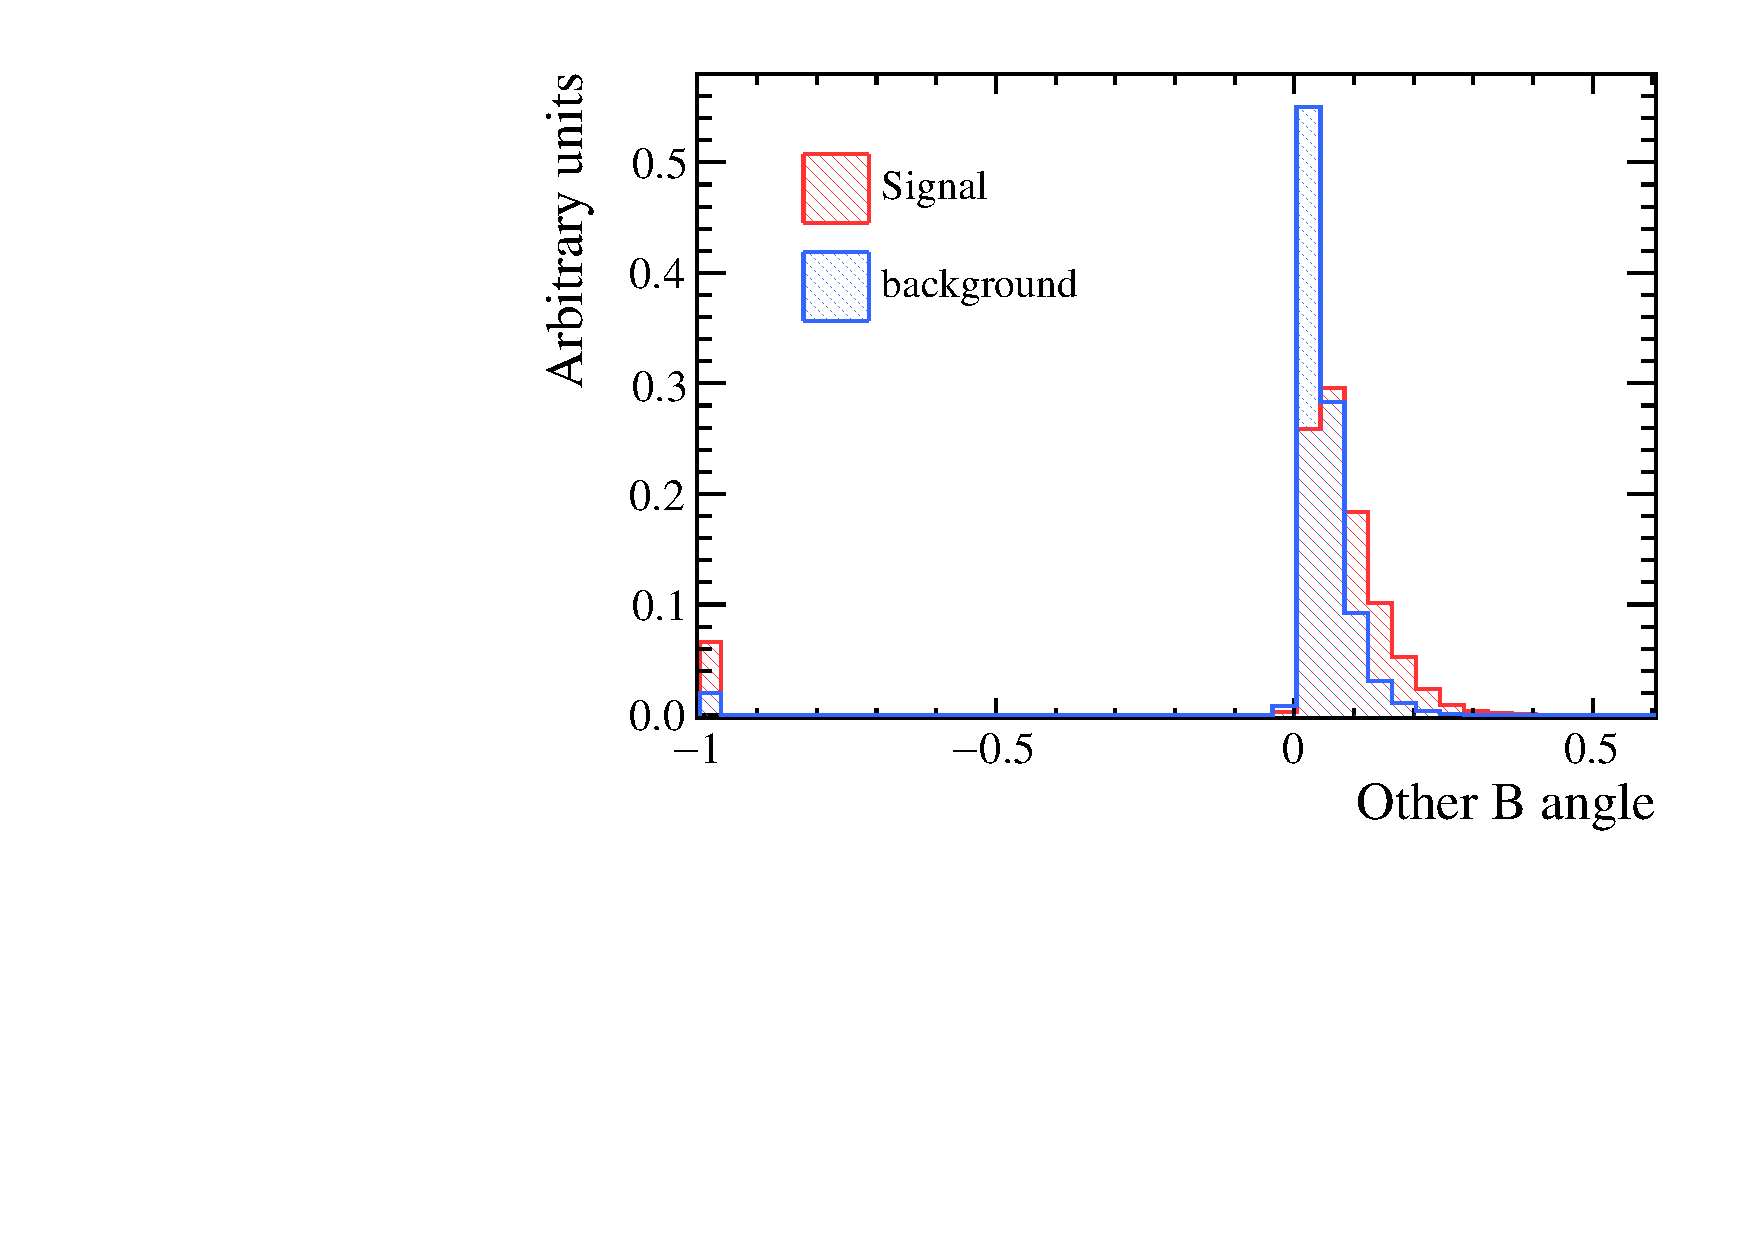
\includegraphics[width=0.49\textwidth]{./Figs/Appendix2/B_other_angle.pdf}
  \caption{The distributions of the input variables used in the adaptive boost and uBoost BDTs for \bsmumu and \bbbarmumux 2012 simulated decays.}
  \label{fig:myBDTvars}
\end{figure}



\begin{figure}[htbp]
  \centering
    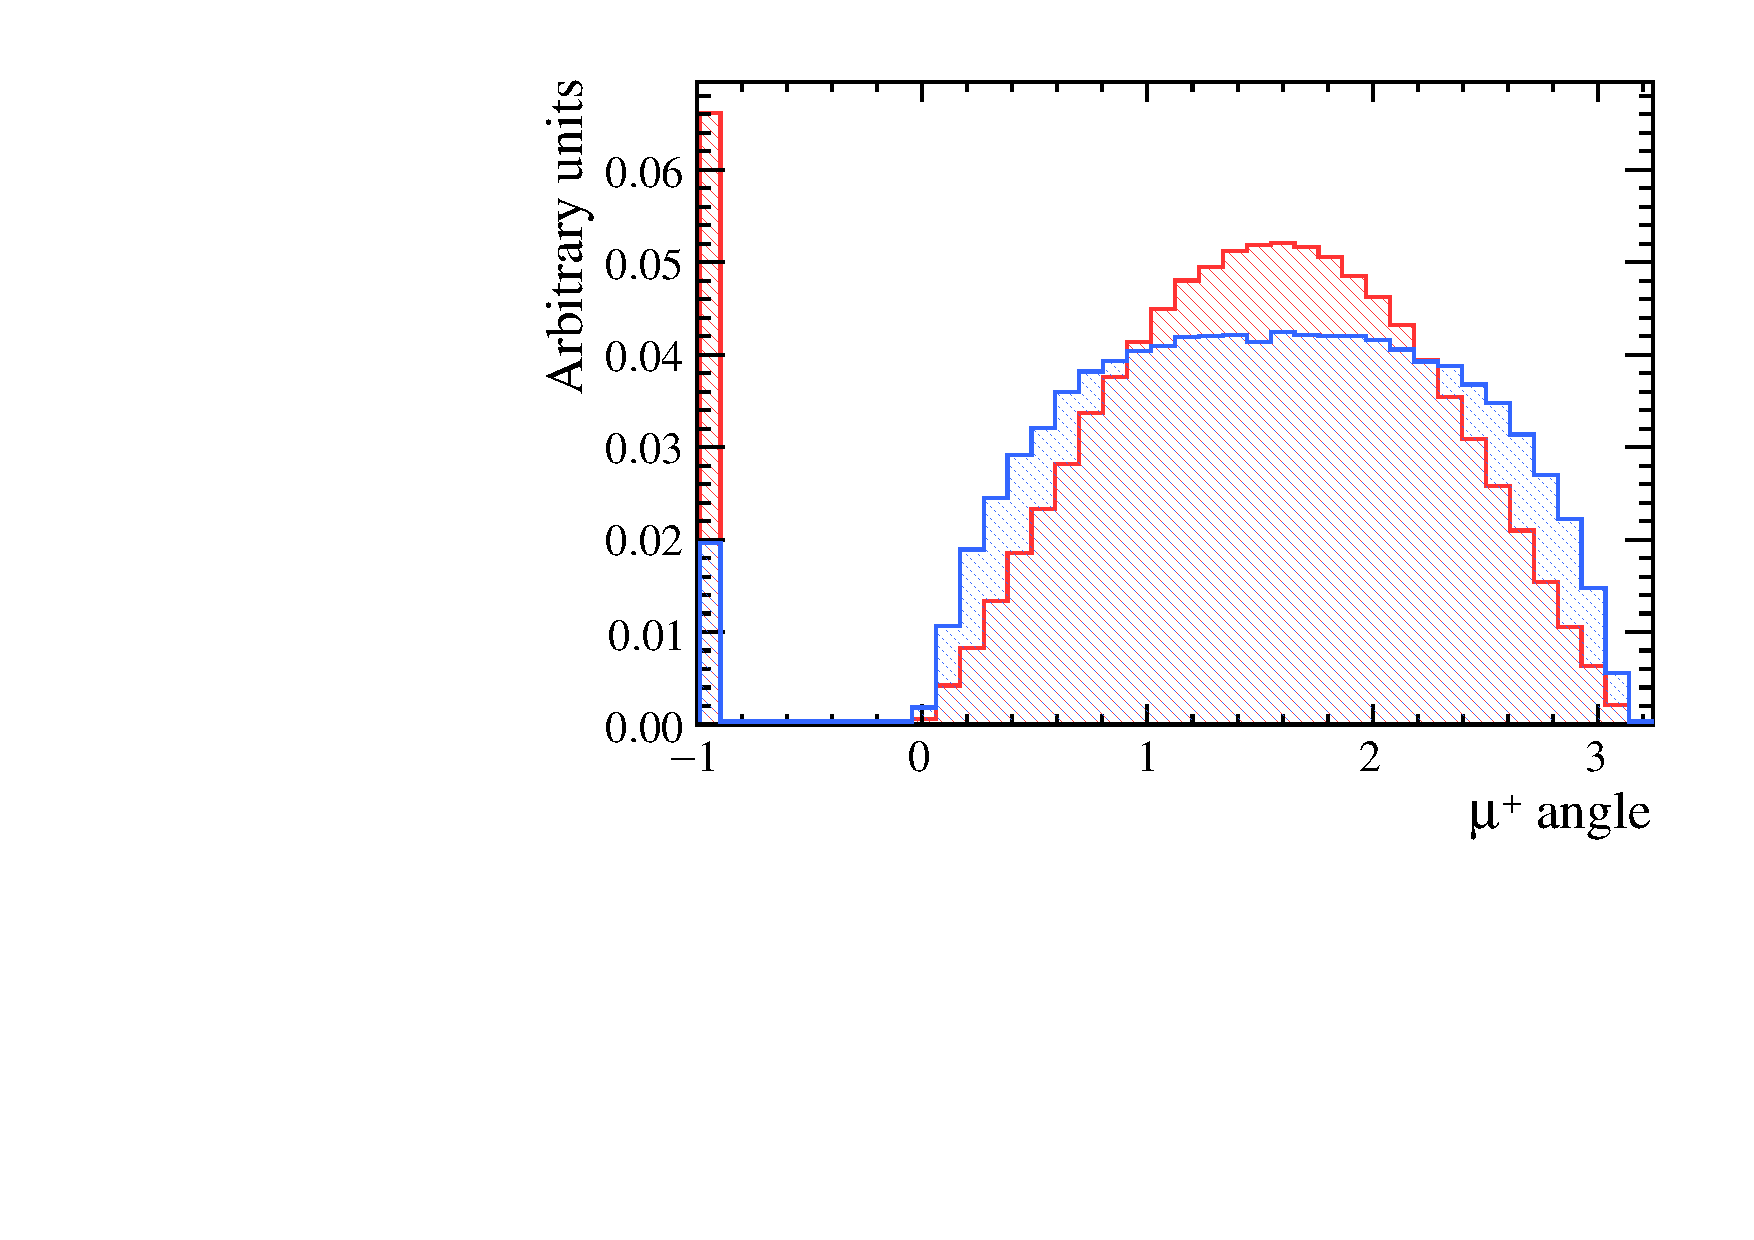
\includegraphics[width=0.49\textwidth]{./Figs/Appendix2/muon_angle.pdf}
    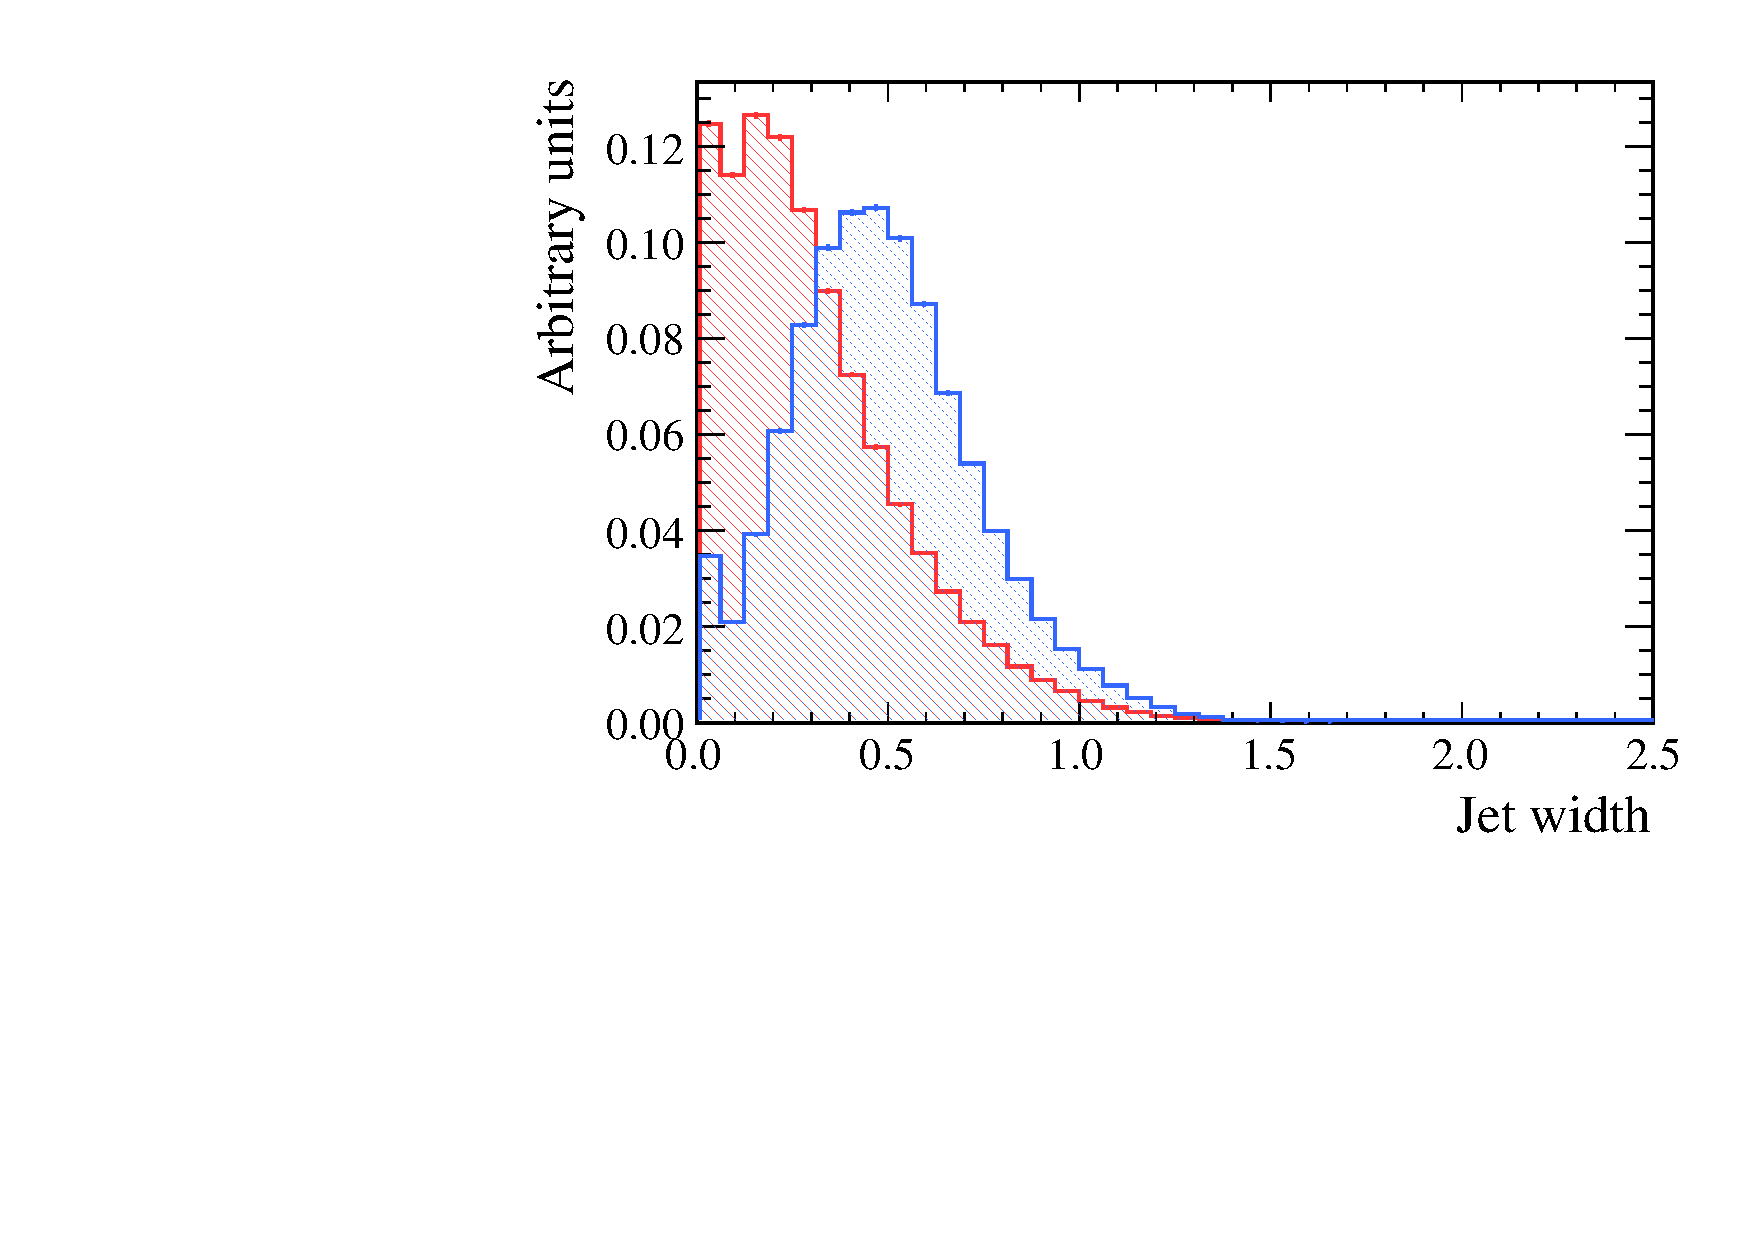
\includegraphics[width=0.49\textwidth]{./Figs/Appendix2/jet_width.pdf}
    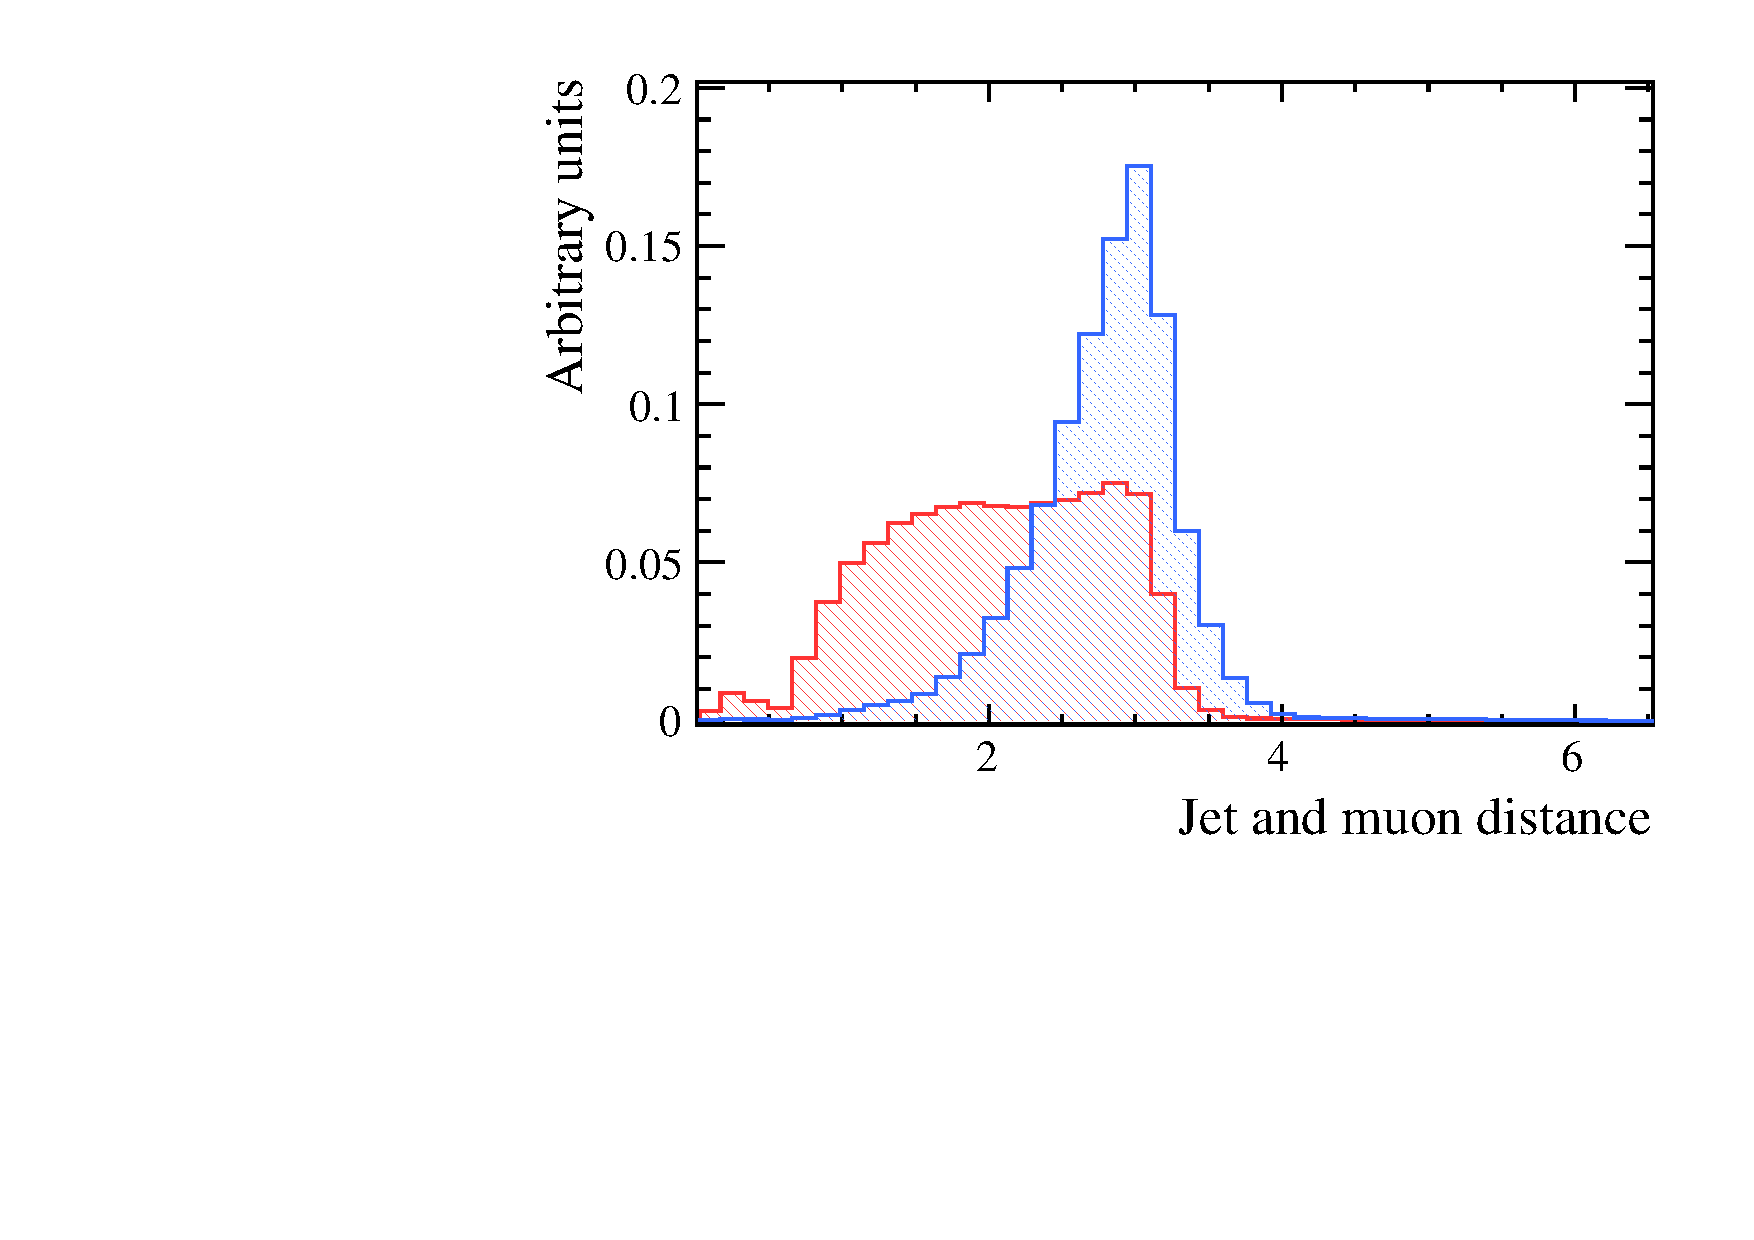
\includegraphics[width=0.49\textwidth]{./Figs/Appendix2/jet_daugt_dist.pdf}
    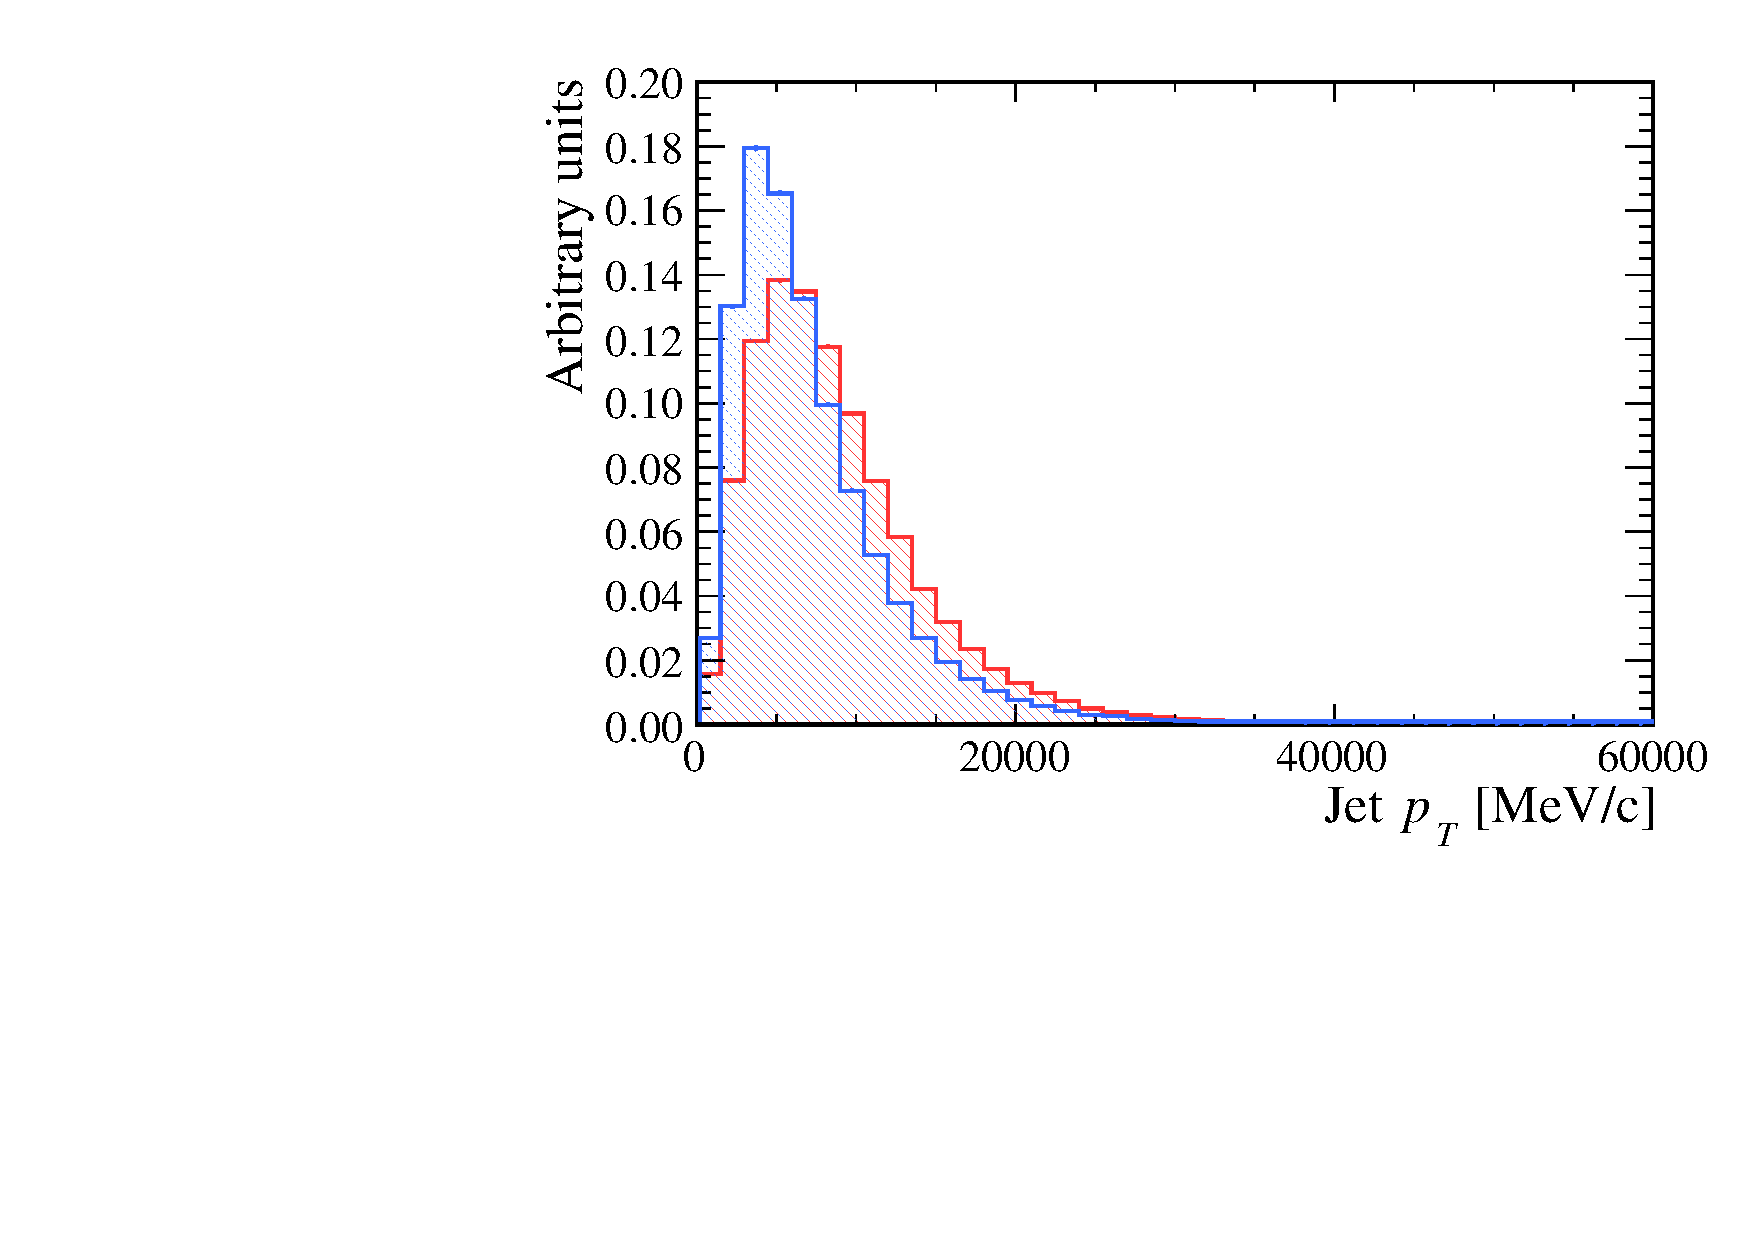
\includegraphics[width=0.49\textwidth]{./Figs/Appendix2/jet_pt.pdf}
    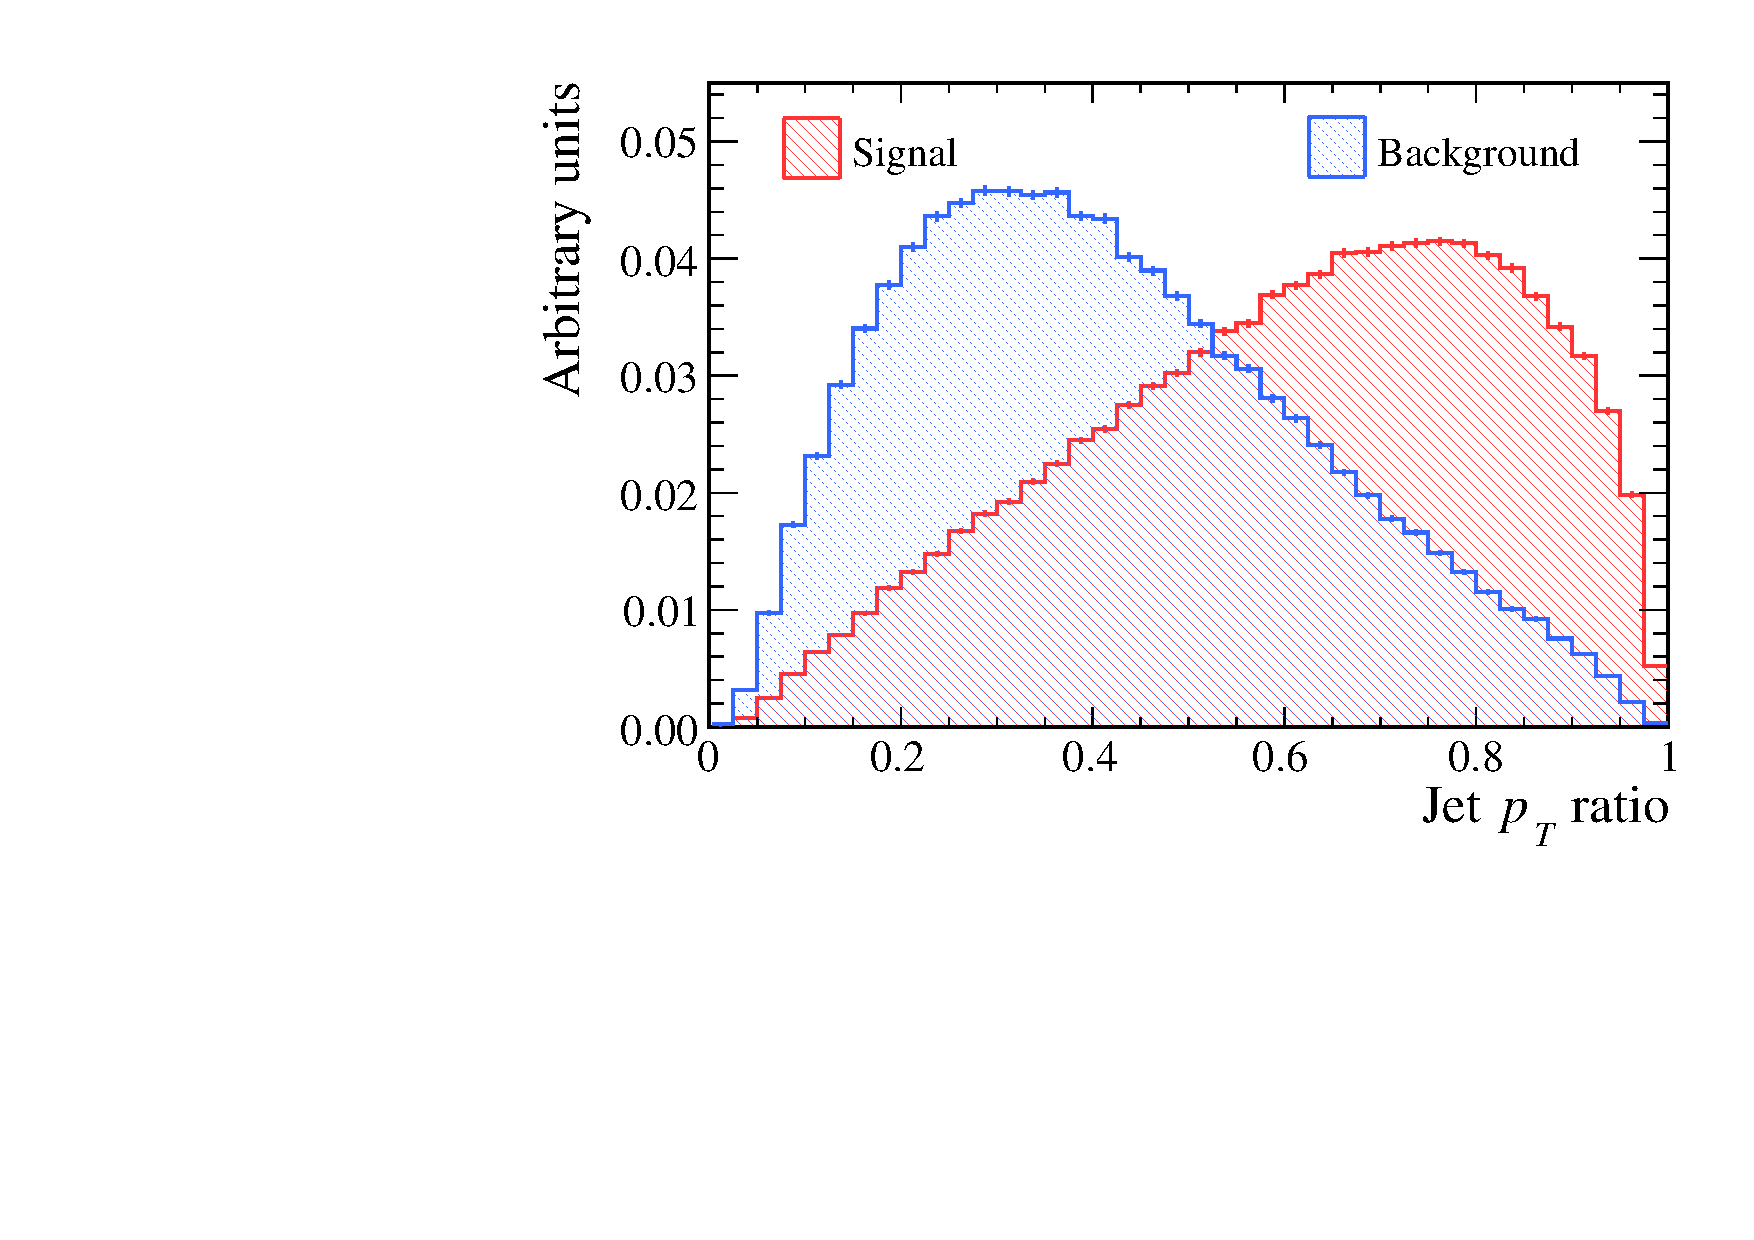
\includegraphics[width=0.49\textwidth]{./Figs/Appendix2/jet_pt_ratio.pdf}
 
  \caption{The distributions of the input variables used in only the uBoost BDT for \bsmumu and \bbbarmumux 2012 simulated decays.}
  \label{fig:myBDTvars}
\end{figure}




\section{Training parameters}
%- The training parmeters used in the final BDTs trained on data are ....
The training parameters discussed in Section~\ref{sec:GeneralBDT} put constraints on how a BDT separates signal and background decays. 
The training parameters used in the adaptive boost BDT were optimised by iterating over different training parameter values and choosing the BDT that gave the best signal significance for identifying \bhh decays in Run~1 data. The computation of the signal significance is described in Section~\ref{sec:dev_BDTs}. %The training parameters were optimised one-by-one in the order NCuts, NTrees, MinNodeSize, MaxDepth the $\beta$, the default TMVA values were taken as the starting point.
The final set of training parameters are given in Table~\ref{tab:ELtrainingparamss}. %{\it I can find the book with this in and add a few more details?}
The training parameters used in the uBoost BDT have not been optimised and are given in Table~\ref{tab:ELtrainingparamss}. The parameter values suggested in reference~\cite{Stevens:2013dya} have been used where it was shown that different training parameters had a small impact of the overall BDT performance. %are given in Table~\ref{}, the parameters are taken from~\ref{} and have no alternative parameters were investigated because little improvment can be gained for this algorithm by altering the training parameters.
\begin{table}[htbp]
\begin{center}
\begin{tabular}{llll}
\toprule \toprule
\multicolumn{2}{c}{Adaptive Boost BDT} & \multicolumn{2}{c}{uBoost BDT} \\ \midrule
Parameter & Value & Parameter & Value\\ \midrule
nTrees & 1000 &  nTrees & 100\\
%nEventsMin & 400 \\                                                                                                                                                                
MinNodeSize & 5$\%$ & nEventsMin & 100 \\
MaxDepth & 3 & MaxDepth & 4 \\
%NNodesMax = 100000 \\                                                                                                                                                              
$\beta$ & 0.1 & $\beta$ & 1.0 \\
nCuts & 30 & nCuts & 200 \\
\bottomrule \bottomrule
\end{tabular}
\vspace{0.7cm}
\caption{Training parameters used to specify the training of the adaptive boost and uBoost BDT.}
\label{tab:ELtrainingparamss}
\end{center}
\vspace{-1.0cm}
\end{table}


\section{Overtraining test}
%- Overtaining of the BDTs
As discussed in Section~\ref{sec:GeneralBDT}, it is important that BDTs are not overtrained. %To test this the signal and background samples are split into two and half of the signal and background samples are used to train a BDT, the BDT is then applied to the other half of the signal and background samples. 
%The BDT output value is evaluated for each decay in the sample and the output values are compared for both s
To test this assumption the signal and background samples are both split in two, to create a training set and a testing set.
A BDT is trained using the training set, and the BDT is then applied to both the training and testing sets. The distribution of BDT output values for signal and background decays in the training and testing sets are compared. If the BDT is overtrained the response of the BDT will be quite different for the training and testing sets for signal and background decays. However, if the BDT is not overtrained the distributions will be similar for the training and testing sets. 

Figure~\ref{fig:ELBDTovertrain} shows the results of this test where the responses for the training and testing samples lie on top of each other. Therefore, neither the uBoost BDT or the adaptive boosting BDT developed for the effective lifetime measurement are overtrained. The same test was performed for the global BDT developed of the \BFm and the global BDT is not overtrained.  

%The output values of the BDT for the set of decays used in training is compared to the output values of the set of decays not used in training. 
\begin{figure}[htbp]
   \centering
        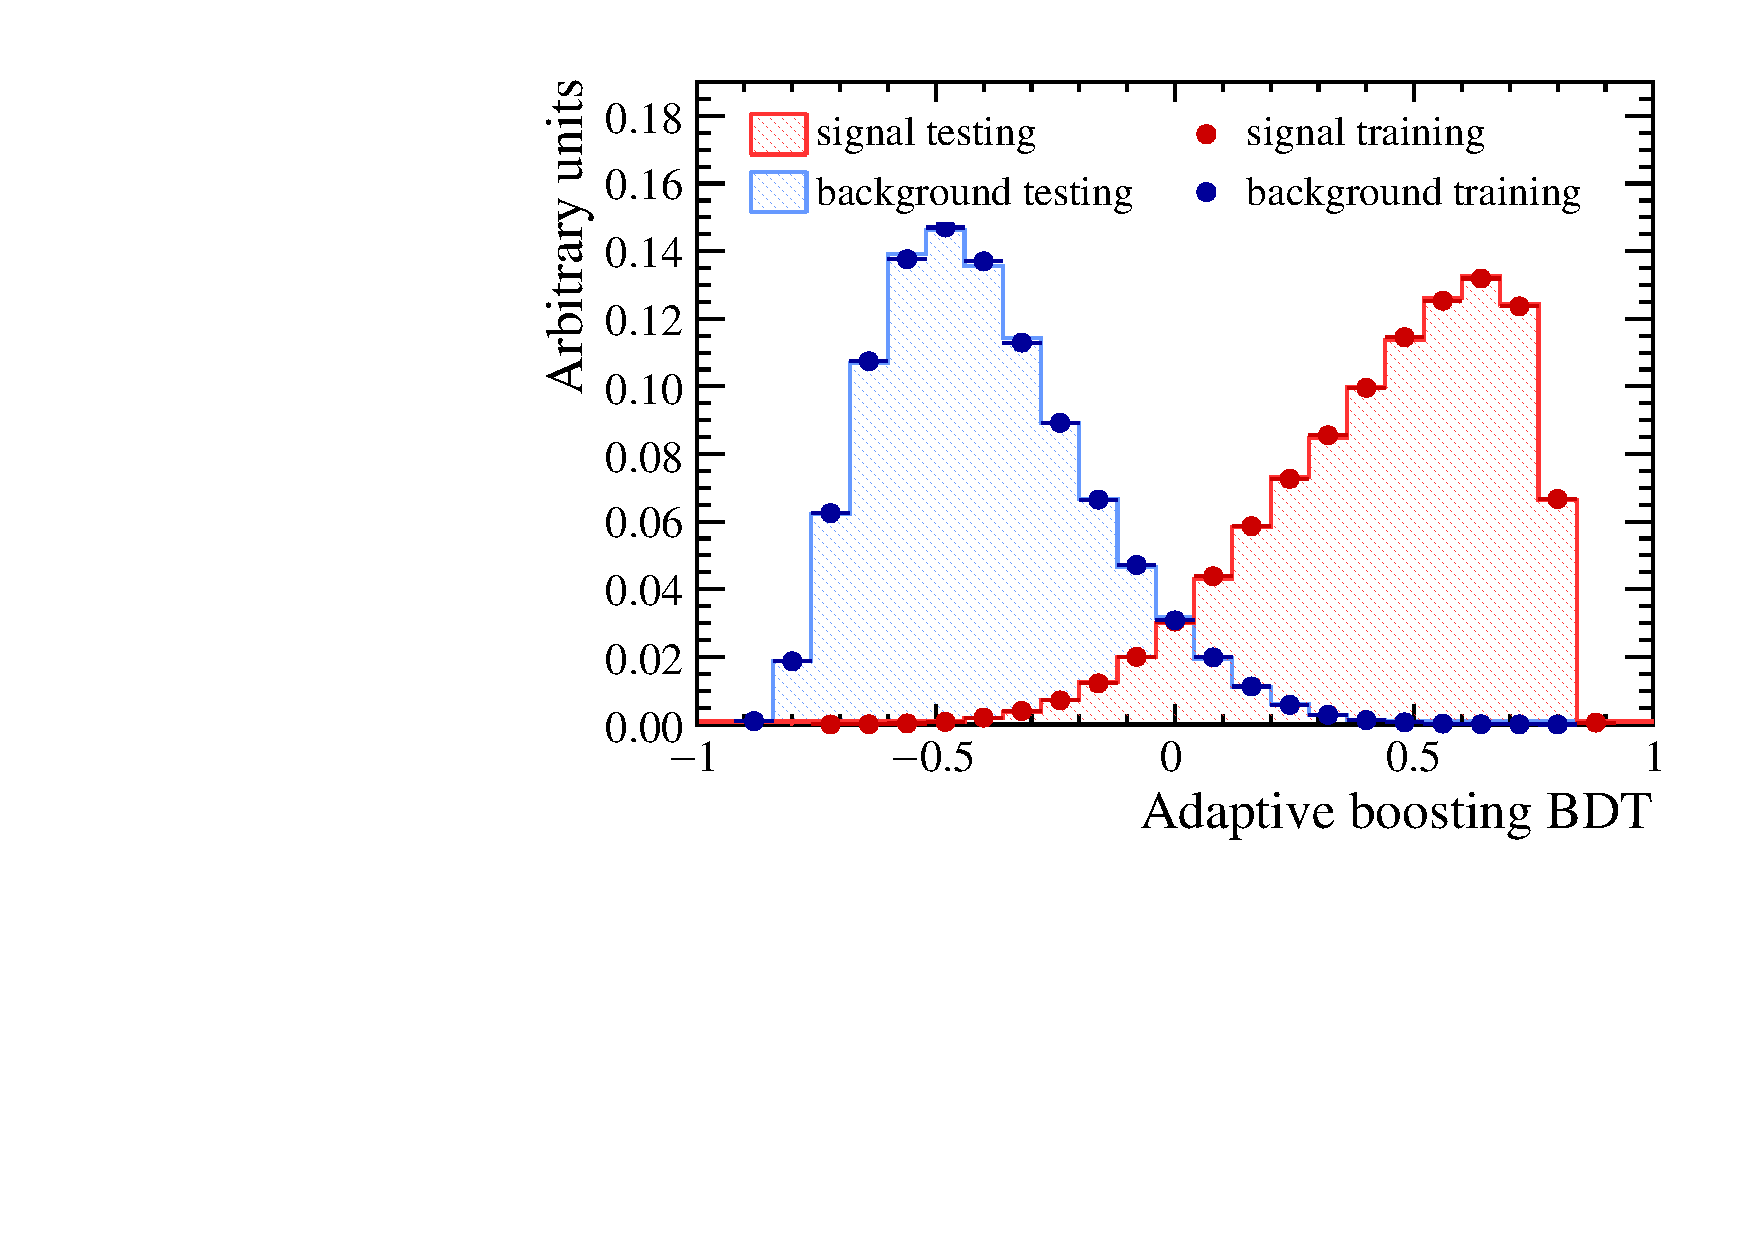
\includegraphics[width=0.49\textwidth]{./Figs/Appendix2/Overtainting_BDT.pdf}
        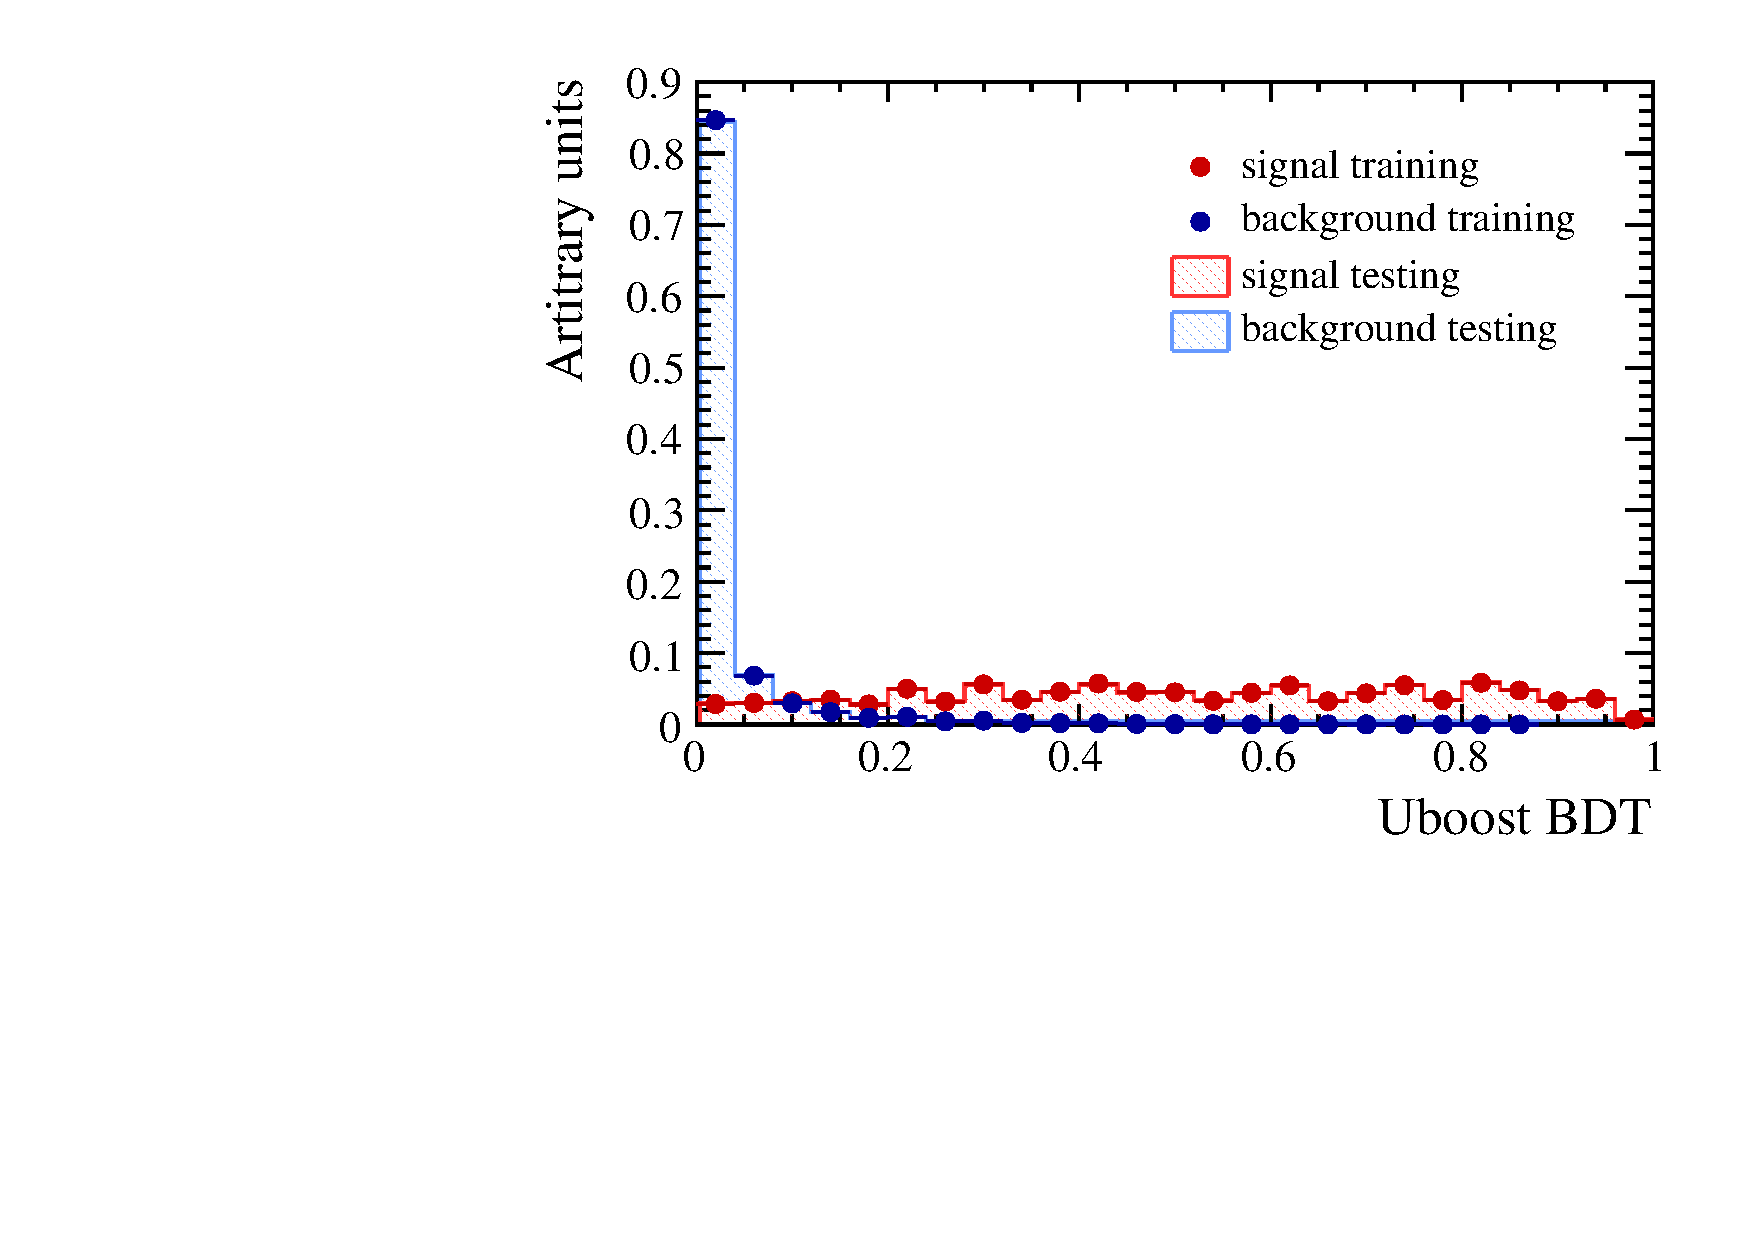
\includegraphics[width=0.49\textwidth]{./Figs/Appendix2/uBoost_overtraining.pdf}

    \caption{BDT response for training and testing samples of signal and background decays for a) the adaptive boost BDT and b) the uBoost BDT. }
    \label{fig:ELBDTovertrain}
\end{figure}



%\begin{figure}[htbp]
%   \centering
%        \includegraphics[width=0.6\textwidth]{./Figs/Appendix2/}
%    \caption{BDT response for training and testing samples of signal and background decays for the global BDT~cite{}. }
%    \label{fig:BFBDTovertrain}
%\end{figure}



